%% 
%% Copyright 2007, 2008, 2009 Elsevier Ltd
%% 
%% This file is part of the 'Elsarticle Bundle'.
%% ---------------------------------------------
%% 
%% It may be distributed under the conditions of the LaTeX Project Public
%% License, either version 1.2 of this license or (at your option) any
%% later version.  The latest version of this license is in
%%    http://www.latex-project.org/lppl.txt
%% and version 1.2 or later is part of all distributions of LaTeX
%% version 1999/12/01 or later.
%% 
%% The list of all files belonging to the 'Elsarticle Bundle' is
%% given in the file `manifest.t\textbf{xt}'.
%% 

%% Template article for Elsevier's document class `elsarticle'
%% with numbered style bibliographic references
%% SP 2008/03/01

\documentclass[preprint,review,11pt]{elsarticle}

%% Use the option review to obtain double line spacing
%%\documentclass[authoryear,preprint,review,12pt]{elsarticle}

%% Use the options 1p,twocolumn; 3p; 3p,twocolumn; 5p; or 5p,twocolumn
%% for a journal layout:
%% \documentclass[final,1p,times]{elsarticle}
%% \documentclass[final,1p,times,twocolumn]{elsarticle}
%% \documentclass[final,3p,times]{elsarticle}
%% \documentclass[final,3p,times,twocolumn]{elsarticle}
%% \documentclass[final,5p,times]{elsarticle}
%% \documentclass[final,5p,times,twocolumn]{elsarticle}

%% For including figures, graphicx.sty has been loaded in
%% elsarticle.cls. If you prefer to use the old commands
%% please give \usepackage{epsfig}

%% The amssymb package provides various useful mathematical symbols
\usepackage{amssymb}
%% The amsthm package provides extended theorem environments
%% \usepackage{amsthm}

%% The lineno packages adds line numbers. Start line numbering with
%% \begin{linenumbers}, end it with \end{linenumbers}. Or switch it on
%% for the whole article with \linenumbers.
%% \usepackage{lineno}

\usepackage{fullpage}
\usepackage{amsfonts}
\usepackage{graphicx}
\usepackage{amsmath}
\usepackage{indentfirst}
\usepackage[version=3]{mhchem} % Formula subscripts using \ce{}
\usepackage[T1]{fontenc}       % Use modern font encodings

\usepackage{float}
\usepackage{chemfig}
\usepackage{longtable}
\usepackage{array}
\usepackage{cellspace}
\usepackage{palatino}
%\usepackage{breqn}
\usepackage{amssymb}
\usepackage{verbatim}
\usepackage[colorlinks=true,citecolor=blue,linkcolor=blue]{hyperref}
\usepackage{siunitx}
\usepackage{xr}
\usepackage{adjustbox}
\usepackage{lscape}

\usepackage{setspace}

%%% Old arguments
%\usepackage{graphicx}
%% uncomment according to your operating system:
%% ------------------------------------------------
%\usepackage[latin1]{inputenc}    %% european characters can be used (Windows, old Linux)
%%\usepackage[utf8]{inputenc}     %% european characters can be used (Linux)
%%\usepackage[applemac]{inputenc} %% european characters can be used (Mac OS)
%% ------------------------------------------------
%\usepackage{authblk}
%\usepackage[superscript]{cite}
%\usepackage[document]{ragged2e}
%\usepackage[T1]{fontenc}   %% get hyphenation and accented letters right
%\usepackage{mathptmx}      %% use fitting times fonts also in formulas
%% do not change these lines:
%\pagestyle{empty}                %% no page numbers!
%\usepackage[left=35mm, right=35mm, top=15mm, bottom=20mm, noheadfoot]{geometry}
%%% please don't change geometry settings!
%
%\usepackage{fullpage}
%\usepackage{amsfonts}
%\usepackage{graphicx}
%\usepackage{float}
%\usepackage{amsmath}
%\usepackage{chemfig}
%\usepackage{indentfirst}
%\usepackage{longtable}
%\usepackage{array}
%\usepackage{cellspace}
%\usepackage{palatino}
%%\usepackage{breqn}
%\usepackage{amssymb}
%\usepackage{verbatim}
%\usepackage[colorlinks=true,citecolor=blue,linkcolor=blue]{hyperref}
%\usepackage{siunitx}
%\usepackage{xr}

%% italicized boldface for math (e.g. vectors)
%\newcommand{\bfv}[1]{{\mbox{\boldmath{$#1$}}}}
%% non-italicized boldface for math (e.g. matrices)
%\newcommand{\bfm}[1]{{\bf #1}}          
%
%%\newcommand{\bfm}[1]{{\mbox{\boldmath{$#1$}}}}
%%\newcommand{\bfm}[1]{{\bf #1}}
%\newcommand{\expect}[1]{\left \langle #1 \right \rangle} % <.> for denoting expectations over realizations of an experiment or thermal averages
%
%\newcommand{\var}[1]{{\mathrm var}{(#1)}}
%\newcommand{\x}{\bfv{x}}
%\newcommand{\y}{\bfv{y}}
%\newcommand{\f}{\bfv{f}}
%
%\newcommand{\hatf}{\hat{f}}
%
%\newcommand{\bTheta}{\bfm{\Theta}}
%\newcommand{\btheta}{\bfm{\theta}}
%\newcommand{\bhatf}{\bfm{\hat{f}}}
%\newcommand{\Cov}[1] {\mathrm{cov}\left( #1 \right)}
%\newcommand{\T}{\mathrm{T}}                                % T used in matrix transpose
%
%\newcommand\blfootnote[1]{%
%	\begingroup
%	\renewcommand\thefootnote{}\footnote{#1}%
%	\addtocounter{footnote}{-1}%
%	\endgroup
%}

\newenvironment{myequation}{%
	\addtocounter{equation}{-1}
	\refstepcounter{defcounter}
	\renewcommand\theequation{SI.\thedefcounter}
	\begin{equation*}}
{\end{equation*}}

\renewcommand{\thefigure}{SI.\arabic{figure}}

\renewcommand{\thepage}{SI.\arabic{page}}

\renewcommand{\thesection}{SI.\Roman{section}}

\renewcommand{\thetable}{SI.\Roman{table}}

\makeatletter
\newcommand*{\addFileDependency}[1]{% argument=file name and extension
	\typeout{(#1)}
	\@addtofilelist{#1}
	\IfFileExists{#1}{}{\typeout{No file #1.}}
}
\makeatother

\newcommand*{\myexternaldocument}[1]{%
	\externaldocument{#1}%
	\addFileDependency{#1.tex}%
	\addFileDependency{#1.aux}%
}

\myexternaldocument{Special_issue_manuscript}

% The figures are in a figures/ subdirectory.
\graphicspath{{figures/}}

\journal{Fluid Phase Equilibria}

\begin{document}
	
	\begin{frontmatter}
		
		%% Title, authors and addresses
		
		%% use the tnoteref command within \title for footnotes;
		%% use the tnotetext command for theassociated footnote;
		%% use the fnref command within \author or \address for footnotes;
		%% use the fntext command for theassociated footnote;
		%% use the corref command within \author for corresponding author footnotes;
		%% use the cortext command for theassociated footnote;
		%% use the ead command for the email address,
		%% and the form \ead[url] for the home page:
		%% \title{Title\tnoteref{label1}}
		%% \tnotetext[label1]{}
		%% \author{Name\corref{cor1}\fnref{label2}}
		%% \ead{email address}
		%% \ead[url]{home page}
		%% \fntext[label2]{}
		%% \cortext[cor1]{}
		%% \address{Address\fnref{label3}}
		%% \fntext[label3]{}
		
		\title{Supporting Information: Improvements and limitations of Mie $\lambda$-6 potential for prediction of saturated and compressed liquid viscosity}
		%\title{Improvements and limitations of Mie $\lambda$-6 potential for prediction of liquid viscosity at saturation and elevated pressures}
		%\title{Improvements and limitations of Mie $\lambda$-6 force fields for predicting liquid shear viscosity at saturation and elevated pressures}
		
		%% use optional labels to link authors explicitly to addresses:
		%% \author[label1,label2]{}
		%% \address[label1]{}
		%% \address[label2]{}
		
		\author{Richard A. Messerly}
		\ead{richard.messerly@nist.gov}
		\address{Thermodynamics Research Center, National Institute of Standards and Technology, Boulder, Colorado, 80305}
		
		\author{Michelle C. Anderson}
		\ead{michelle.anderson@nist.gov}
		\address{Thermodynamics Research Center, National Institute of Standards and Technology, Boulder, Colorado, 80305}
		
		\author{S. Mostafa Razavi}
		\address{Department of Chemical and Biomolecular Engineering, The University of Akron, Akron, Ohio, 44325-3906}
        \ead{sr87@zips.uakron.edu}
		
		\author{J. Richard Elliott}
		\address{Department of Chemical and Biomolecular Engineering, The University of Akron, Akron, Ohio, 44325-3906}
		\ead{elliot1@uakron.edu}
		
		%		
		%	\thispagestyle{empty}
		%	%make title bold and 14 pt font (Latex default is non-bold, 16 pt)
		%	\title{\Large \textbf{Transferability of Mie $\lambda$-6 force fields for predicting liquid shear viscosity at saturation and elevated pressures}}
		%
		%	\date{} % <--- leave date empty
		%	\maketitle\thispagestyle{empty} %% <-- you need this for the first page
		%	\begin{center}
		%		\title{\textbf{ABSTRACT}}\centering{}
		%	\end{center}
		%	\justify
		%	
		%	\author{Richard A. Messerly}
		%	\email{richard.messerly@nist.gov}
		%	\affiliation{Thermodynamics Research Center, National Institute of Standards and Technology, Boulder, Colorado, 80305}
		%	
		%	\author{Michael R. Shirts}
		%	\email{michael.shirts@colorado.edu}
		%	\affiliation{Department of Chemical and Biological Engineering, University of Colorado, Boulder, Colorado, 80309}
		%	
		%	\author{Andrei F. Kazakov}
		%	\email{andrei.kazakov@nist.gov}
		%	\affiliation{Thermodynamics Research Center, National Institute of Standards and Technology, Boulder, Colorado, 80305}
		
%		\begin{abstract}
%			%% Text of abstract
%			%%% MCA abstract:
%%			To determining reliable methodologies and models for the estimation of viscosities, equilibrium molecular dynamics simulations for normal and branched alkanes ranging from two to sixteen carbons were performed with the GROMACS package. Viscosities along the liquid/vapor saturation curve and at 293 K and high-pressure conditions were generated using the TraPPE, Potoff, and TAMie force fields. Viscosities were calculated from simulations using the Green-Kubo method. Reliable data and uncertainties were determined by performing many replicate simulations and analyzing the data distributions. Potoff and TAMie, modern force fields making use of the Mie $\lambda$-6 (the generalized Lennard-Jones 12-6 potential), outperform the older TraPPE force field which makes use of the traditional Lennard-Jones 12-6 potential. Simulations carried out with the Potoff or TAMie potentials more closely follow trends in viscosity. The TraPPE force field consistently under predicts viscosities. Although simulations with the Potoff force field overestimate viscosity with respect to density, a fortuitous cancellation of errors results in good prediction of viscosity with respect to pressure. The performance of the TAMie force field is usually better than TraPPE but slightly worse than Potoff. All force fields perform somewhat better for normal alkanes than for branched alkanes and the differences in performance between force fields is more noticeable in the case of normal alkanes.
%		
%		%%% JRE abstract:	
%%			While many common force fields are developed based only liquid density and heat of vaporization at 25 C, several more recent force fields have taken into account vapor pressure and liquid density over substantial portions of the coexistence curve for multiple compounds simultaneously, enhancing transferability. This manuscript explores the hypothesis that greater accuracy in characterizing the coexistence properties may lead to greater accuracy for viscosity predictions. Three united atom force fields are considered in detail: the TraPPE-UA model of Siepmann and coworkers, the TAMie model of Gross and coworkers, the AUA4 model of Ungerer and coworkers, and the TraMie model of Potoff and coworkers. Equilibrium molecular dynamics simulations are performed in the NVT ensemble using the Green-Kubo method for viscosity characterization. Simulations are performed for linear alkanes with three to twelve carbons and branched alkanes with four to nine carbons.  Simulation conditions follow the saturated liquid from reduced temperatures of 0.5-0.9 and along key isotherms in the dense liquid region. In general, the more accurate force fields for coexistence properties do indeed predict viscosity more accurately. For saturated liquids, both the TraMie and TAMie models provide roughly 10 \% accuracy for linear alkanes, while deviations are closer to 20-30 \% for AUA4 and TraPPE-UA models. For branched alkanes the behavior is more complicated but TraMie still provides roughly 15 \% accuracy while TraPPE-UA adn AUA4 accuracy is around 25-35 \% deviations. TAMie force fields for branched alkanes were unavailable at thee time of this study.For compressed liquids,  the Mie potential models perform better once again, but tend to overestimate the viscosity at very high pressures. Coincidentally, these models also tend to overestimate the pressure, such that plots of viscosity vs. pressure are  accurate to within about 10 \% up to 200 MPa. Experimental viscosity data tend to be sparse above 200 MPa, but accurate predictions are obtained for propane to 1000 MPa. Uncertainty estimates increase substantially for high pressures at low reduced temperatures. Nevertheless, a prediction is made for the viscosity of 2,2,4, trimethylhexane at 293K and 1000 MPa, in compliance with the guidelines of the 10th IFPSC. In the course of the study, the sensitivity to bonded and non-bonded interactions is observed and several suggestions are made for future force field developments.
%			
%%			While many common force fields are developed based on liquid density and heat of vaporization at room temperature, several more recent force fields have taken into account saturated vapor pressure and saturated liquid density over substantial portions of the vapor-liquid coexistence curve for multiple compounds simultaneously, enhancing transferability. 
%
%			Over the past decade, the Mie $\lambda$-6 (generalized Lennard-Jones) potential has grown in popularity due to its improved accuracy for predicting vapor-liquid coexistence compared to the traditional Lennard-Jones 12-6. This manuscript explores the hypothesis that greater accuracy in characterizing the coexistence properties may lead to greater accuracy for viscosity predictions. Four united atom force fields are considered in detail: the TraPPE-UA model of Siepmann and coworkers, the TAMie model of Gross and coworkers, the AUA4 model of Ungerer and coworkers, and the model of Potoff and coworkers. Equilibrium molecular dynamics simulations are analyzed using the Green-Kubo method for viscosity characterization. Simulations are performed for linear alkanes with two to twenty-two carbons and branched alkanes with four to nine carbons. Simulation conditions follow the saturated liquid from reduced temperatures of 0.5 to 0.85 and along the 293 K isotherm in the dense liquid region. 
%			
%			In general, the more accurate force fields for coexistence properties do indeed predict viscosity more accurately. For saturated liquids, both the Potoff and TAMie models provide roughly 10 \% accuracy for linear alkanes, while deviations are closer to 20 to 50 \% for TraPPE-UA. For branched alkanes, the behavior is more complicated but Potoff still provides roughly 15 to 20 \% accuracy, while the TAMie force field results in deviations of 20 to 40 \%, and TraPPE-UA has deviations of approximately 25 to 60 \%. The AUA4 deviations are 10 to 20 \% for ethane and 30 to 60 \% for 2,2-dimethylpropane, the only compounds tested with the AUA4 force field. The TraPPE-2 deviations for ethane are similar to those using the original TraPPE force field, namely, between 10 and 20 \%. The percent deviations for each compound and force field tend to increase with decreasing temperature, with the exception of the Potoff deviations for propane, which are nearly constant to the triple point temperature. 
%			
%			For compressed liquids, the Mie-based potential models perform better once again than the Lennard-Jones-based force fields, but tend to overestimate the viscosity at very high densities. As the Potoff and TAMie models also tend to overestimate the pressure at high densities, a fortuitous cancellation of errors leads to predictions of viscosity with respect to pressure that are accurate to within about 10 \%. Experimental viscosity data tend to be sparse above 200 MPa for normal and branched alkanes, however, accurate predictions are obtained for propane to 1000 MPa with the Potoff force field. 
%			
%			%Uncertainties increase substantially for simulations at high pressures and/or low reduced temperatures. 
%			
%			%Nevertheless, a prediction is made for the viscosity of 2,2,4-trimethylpentane at 293K and 1000 MPa. 
%			
%			%, in compliance with the guidelines of the 10th IFPSC. In the course of the study, the sensitivity to bonded and non-bonded interactions is observed and several suggestions are made for future force field developments.
%			
%		\end{abstract}
%		
%		\begin{keyword}
%			%% keywords here, in the form: keyword \sep keyword
%			
%			%% PACS codes here, in the form: \PACS code \sep code
%			
%			%% MSC codes here, in the form: \MSC code \sep code
%			%% or \MSC[2008] code \sep code (2000 is the default)
%			
%			Thermophysical Properties \sep Molecular Simulation \sep Force fields \sep Molecular dynamics \sep Green-Kubo
%			
%		\end{keyword}
		
	\end{frontmatter}	
	
%	Following ``Best Practices'', we compute $\eta$ with several different production times (1, 2, 4, and 8 ns) for select systems to verify that the results are indistinguishable (see Supporting Information). Furthermore, we investigate system size effects by comparing results with 100, 200, 400, and 800 molecules (see Section \ref{Discussion/Limitations}). In addition, we compare fixed and flexible bonds in the Supporting Information.
	
	\section{Input files} \label{Gromacs input files}
	
	We provide example input files for simulating 2,2,4-trimethylpentane at 245 K with the Potoff force field in GROMACS (see attached .gro, .top, and .mdp files). Additionally, all files necessary to generate the results from this study can be found at \newline www.github.com/ramess101/IFPSC\_10.
	
	%	\begin{enumerate}
	%		\item Include all the .gro files
	%		\item Include all the .top file templates
	%		\item Include .mdp files
	%		\item Or we can just include an example and then refer them to the GitHub website
	%	\end{enumerate}
	%	
	
	\newpage
	
	\section{Systems simulated} \label{Systems simulated}
	
	Table \ref{tab:simulations_performed} enumerates the compounds, force fields, and viscosity types simulated in this study.
	
	\begin{table}[h!]
		\caption{Compounds, force fields, and state points. ``X'': simulated, ``O'': not simulated, ``S'' simulated with ``short'' parameters, ``L'' simulated with ``long'' parameters.} \label{tab:simulations_performed}
		\begin{center}
			\begin{tabular}{|c|c|c|c|c|c|c|c|c|}
				\hline
				\multicolumn{1}{|c}{} & \multicolumn{2}{|c}{TraPPE (TraPPE-2)} & \multicolumn{2}{|c|}{Potoff (S/L)} & \multicolumn{2}{|c}{AUA4} & \multicolumn{2}{|c|}{TAMie}  \\ \hline
				Compound & $\eta_{\rm liq}^{\rm sat}$ & $\eta_{\rm liq}^{\rm comp}$ & $\eta_{\rm liq}^{\rm sat}$ & $\eta_{\rm liq}^{\rm comp}$ & $\eta_{\rm liq}^{\rm sat}$ & $\eta_{\rm liq}^{\rm comp}$ & $\eta_{\rm liq}^{\rm sat}$ & $\eta_{\rm liq}^{\rm comp}$ \\ \hline
				ethane & X (X) & X (X) & X & X & X & X & X & X \\ \hline
				propane & X & X & X & X & O & O & X & X \\ \hline
				\textit{n}-butane & X & X & X & X & O & O & X & X \\ \hline
				\textit{n}-octane & X & X & X & X & O & O & X & X \\ \hline
				\textit{n}-dodecane & X & O & X & O & O & O & X & O \\ \hline
				\textit{n}-hexadecane & X & O & X & O & O & O & X & O \\ \hline
				2-methylpropane & X & X & S & S & O & O & X & X \\ \hline
				2-methylbutane & X & X & S & S & O & O & X & X \\ \hline
				2,2-dimethylpropane & X & X & S & S & X & X & O & O \\ \hline
				2,3-dimethylbutane & X & X & S & S & O & O & X & X \\ \hline
				2-methylpentane & X & X & L & L & O & O & X & X \\ \hline
				3-methylpentane & X & X & L & L & O & O & X & X \\ \hline
				2,2,4-trimethylpentane & X & X & L & L & O & O & O & O \\ \hline
			\end{tabular}
		\end{center} 
	\end{table}

	\newpage

    \section{Additional simulation details} \label{Additional simulation details}
    
    Table \ref{tab:thermostats_barostats} lists the integrators, thermostats, and barostats used for each $NPT$ or $NVT$ stage.
    
    \begin{table}[htbp!]
    	\caption{Integrator, thermostat and barostat specifications.} \label{tab:thermostats_barostats}
%    	\begin{center}
    		\begin{tabular}{|p{2.6cm}|c|c|c|c|}
    			\hline
    			& $NPT$ Equil. & $NPT$ Prod. & $NVT$ Equil. & $NVT$ Prod. \\ \hline
    			Integrator & Velocity Verlet & Leap frog & Velocity Verlet & Velocity Verlet \\ \hline 
    			Thermostat & Velocity rescale & Nos{\'e}-Hoover & Nos{\'e}-Hoover & Nos{\'e}-Hoover \\ \hline 
    			Thermostat time-constant (ps) & 1.0 & 1.0 & 1.0 & 1.0 \\ \hline
    			Barostat & Berendsen & Parrinello-Rahman & N/A & N/A \\ \hline
    			Barostat time-constant (ps) & 1.0 & 5.0 & N/A & N/A \\ \hline
    			Barostat compressibility (1/bar) & 4.5E-5 & 4.5E-5 & N/A & N/A \\
    			\hline
    		\end{tabular}
%    	\end{center} 
    \end{table}
    
	\newpage
		
	\section{Simulation time} \label{SI:Simulation time}
	
%	Following ``Best Practices'', we compute $\eta$ with several different production times (1, 2, 4, and 8 ns) for select systems to verify that the results are indistinguishable (see Supporting Information).
	
	For less viscous systems, i.e., saturation and low pressures, a 1 ns simulation is typically sufficient for the Green-Kubo integral to reach a plateau. However, even when there is an apparent plateau, systematic bias in $\eta$ may still exist if the simulation is too short \cite{Maginn2018,Zhang2015}. For this reason, Figure \ref{fig:simulation_time} compares the Green-Kubo integral for simulations with 0.5 ns, 1 ns, 2 ns, and 4 ns. We observe that the estimated viscosity obtained from a 1 ns trajectory is consistent with that from 2 ns and 4 ns simulations. Specifically, a plateau is observed at a similar value of $\eta$ despite the large fluctuations at long times. We also note that 0.5 ns simulations are typically reliable but occasionally the plateau deviates considerably. For these reasons, the results presented in this study were obtained from 1 ns simulations.
	
	\begin{figure}[htb!]
		\centering
		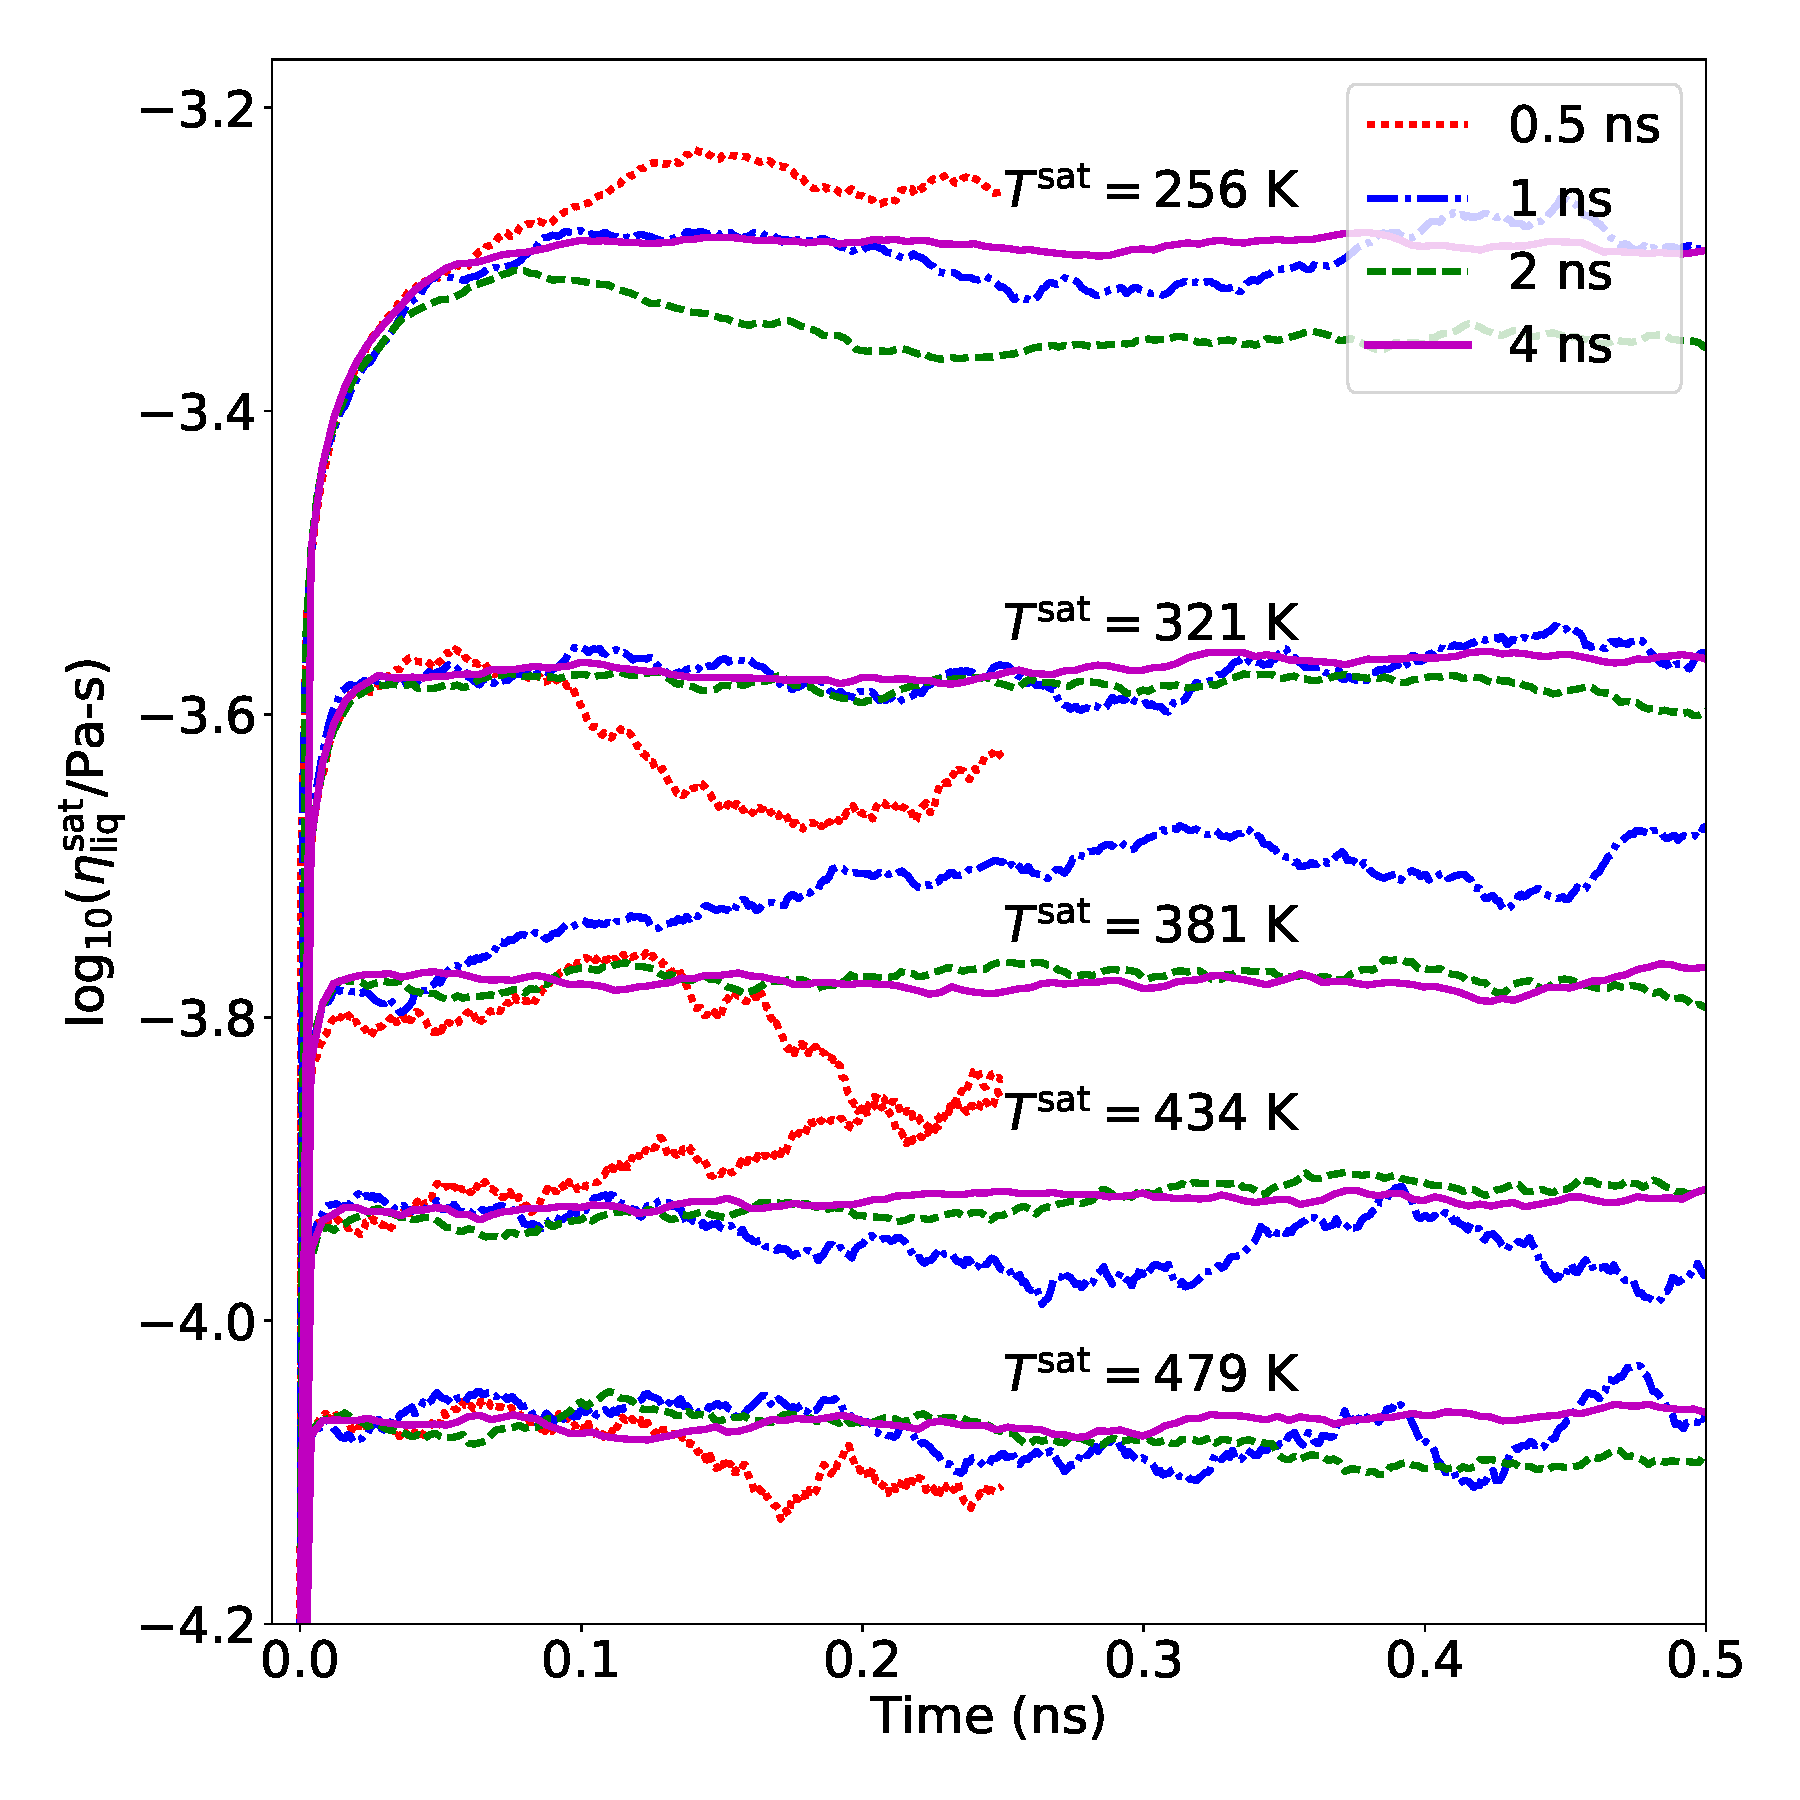
\includegraphics[width=3.2in]{simulation_time}
		\caption{Simulation production time. Simulations were performed for \textit{n}-octane using the TraPPE potential. Colors/line styles denote different simulation times (0.5 ns, 1 ns, 2 ns, and 4 ns).}
		\label{fig:simulation_time}
	\end{figure} 

    For more viscous systems (greater than 0.02 Pa-s) a 1 ns simulation is too short to observe a plateau in the Green-Kubo integral. In these cases, we increase the simulation time to a value between 2 and 8 ns. Due to the increased computational cost of such simulations, we did not perform an exhaustive test with increasing simulation time. Instead, the choice of simulation time was determined primarily by the ability to detect a plateau region. Therefore, it is possible that even longer simulations are required for the most viscous systems. 
    
    Figure \ref{fig:most_viscous} depicts the Green-Kubo integral with respect to time for these highly viscous systems (note that the total simulation time is twice the maximum time plotted). For example, an 8 ns run appears to be sufficient to detect a plateau for 2,2,4-trimethylpentane with Potoff at 750 MPa, while 16 ns are required for 2,2,4-trimethylpentane with Potoff at 1000 MPa. This demonstrates that it is possible to obtain reasonable estimates for systems with viscosities much greater than 0.02 Pa-s. However, the bootstrap uncertainty is significantly larger for these more viscous systems.
    
    % does increase significantly with increasing viscosity.
    
    %  despite this system having a viscosity around 0.08 Pa-s. By contrast, a 1 ns run provides a reasonable plateau for the other two systems with viscosities near 0.02 Pa-s.
    
    \begin{figure}[htb!]
    	\centering
    	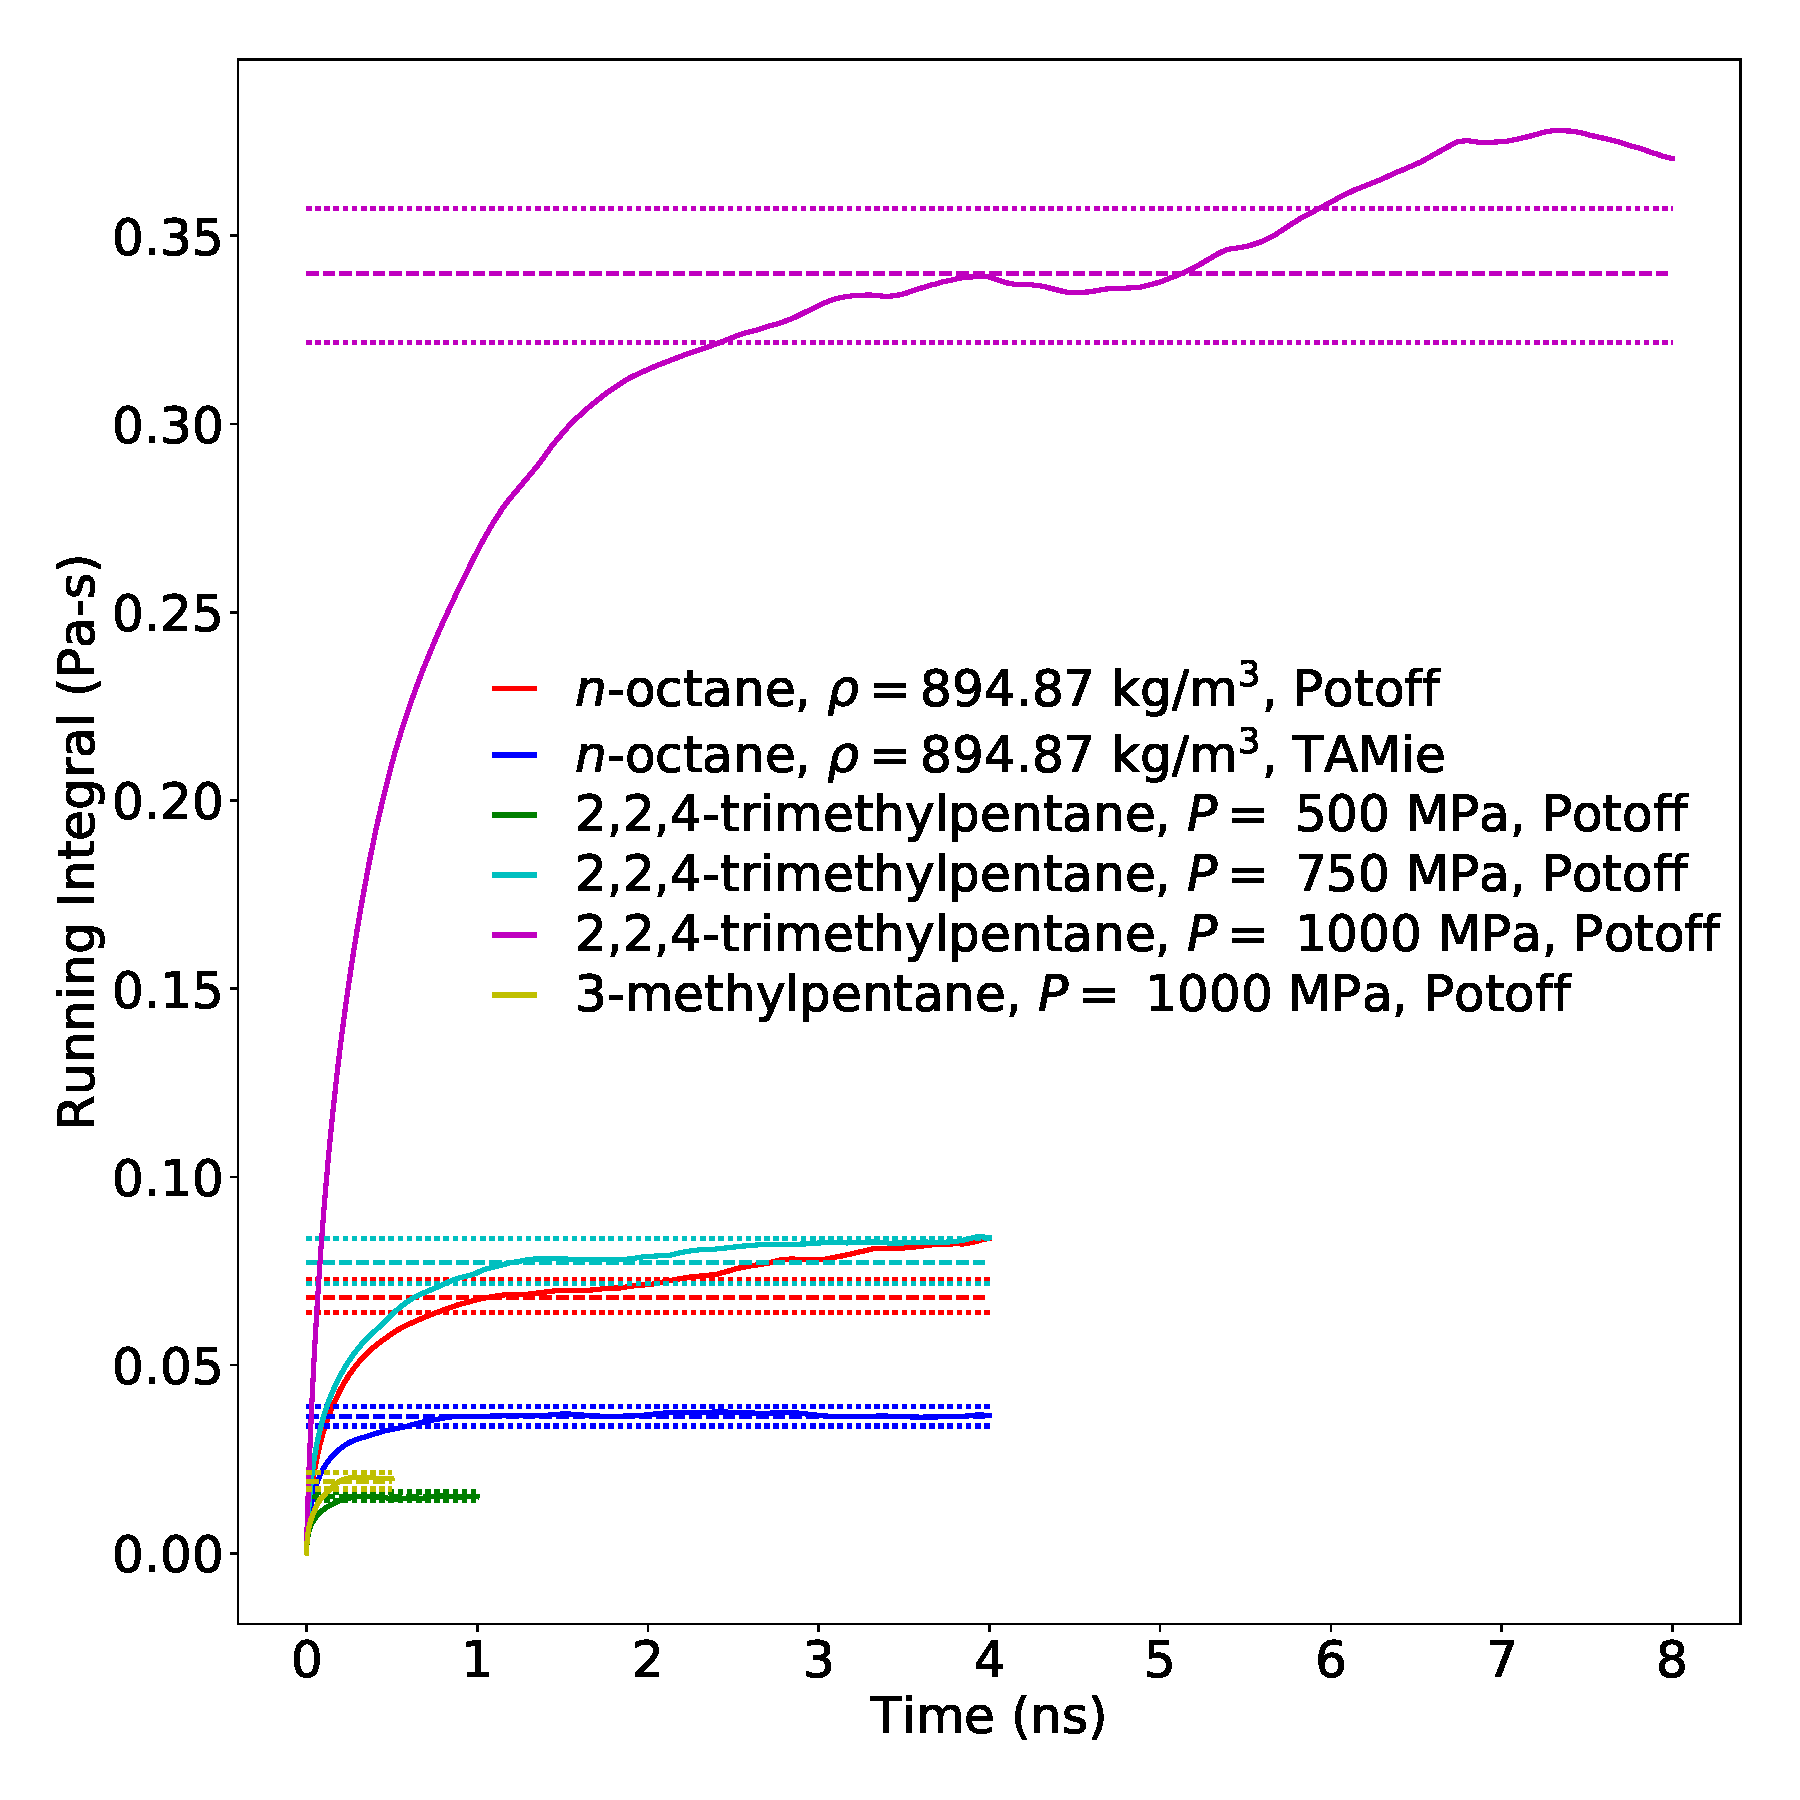
\includegraphics[width=5.2in]{most_viscous_systems.pdf}
    	\caption{Green-Kubo integrals for the most viscous systems studied. Solid lines are the average of $N_{\rm reps}$ replicates. Dashed lines are the estimated $\eta$ value after fitting. Dotted lines represent the 95 \% bootstrapped uncertainties.}
    	\label{fig:most_viscous}
    \end{figure} 
    
    %Simulations performed with Potoff or TAMie force fields.
    
    %, i.e., greater than 100 MPa,
    
%    Due to inherently slow dynamics in highly viscous systems (greater than 0.02 Pa-s), obtaining well-converged Green-Kubo integrals is extremely challenging. Additional replicate simulations can help reduce noise.
%    
%    Storage limitations become a concern with simulations longer than 8 ns due to the frequency at which data are output (every 6 fs). Reading in these files for GROMACS to evaluate the data nearly crippled our computing cluster.
%    
%    Obtaining well-converged Green-Kubo integrals for highly viscous systems (greater than 0.02 Pa-s) is challenging and requires longer simulations.
	
%	\begin{enumerate}
%		\item Verified that 1 ns is long enough for larger compounds
%	\end{enumerate}

	\newpage
	
	\section{Fixed vs flexible bonds} \label{fixed flexible}
	
%    Although static thermodynamic properties (e.g., $\rho_{\rm liq}^{\rm sat}$) are generally insensitive to the choice of fixed or flexible bonds, dynamic properties (e.g., $\eta$) are much more sensitive. For this reason, we test the degree of variability that arises by implementing a harmonic oscillator model.
	
    Although static thermodynamic properties (e.g., $\rho_{\rm liq}^{\rm sat}$) are generally insensitive to the choice of fixed or flexible bonds, dynamic properties (e.g., $\eta$) can be much more sensitive. We perform simulations with flexible bonds to test how sensitive the results presented in this study are to the use of fixed bond-lengths. Specifically, we use the traditional harmonic bond potential:
    \begin{equation} \label{eq:harmonic_bond}
    u^{\rm bond} = \frac{k_{\rm b}}{2} \left(r-r_{\rm eq}\right)^2
    \end{equation}
    where $u^{\rm bond}$ is the bonded potential, $k_{\rm b}$ is the harmonic force constant, and $r_{\rm eq}$ is the equilibrium bond-length. We use an arbitrarily large value for the force constant, $k_{\rm b}/k_{\rm B} = 60.43$ K/pm$^2$, as this should result in a fairly stiff bonded potential, i.e., the bond-lengths should not vary significantly.
    
    %Since the bond-length should not vary significantly, any deviations should not be attributed to the fluctuations in bond-length but rather to the contributions that the bonded forces make to the viscosity. 
    
    Figure \ref{fig:fixed_flexible} demonstrates that the difference between fixed and flexible bonds is negligible in certain cases. However, there is a small, but systematic, deviation towards higher viscosities for the stiff harmonic potential. 
    
    %Bootstrap re-sampling confirms that the LINCS and $k_{\rm b} = $ BLANK results are statistically indistinguishable, while the $k_{\rm b} = $ BLANK is statistically different.

	\begin{figure}[htb!]
		\centering
		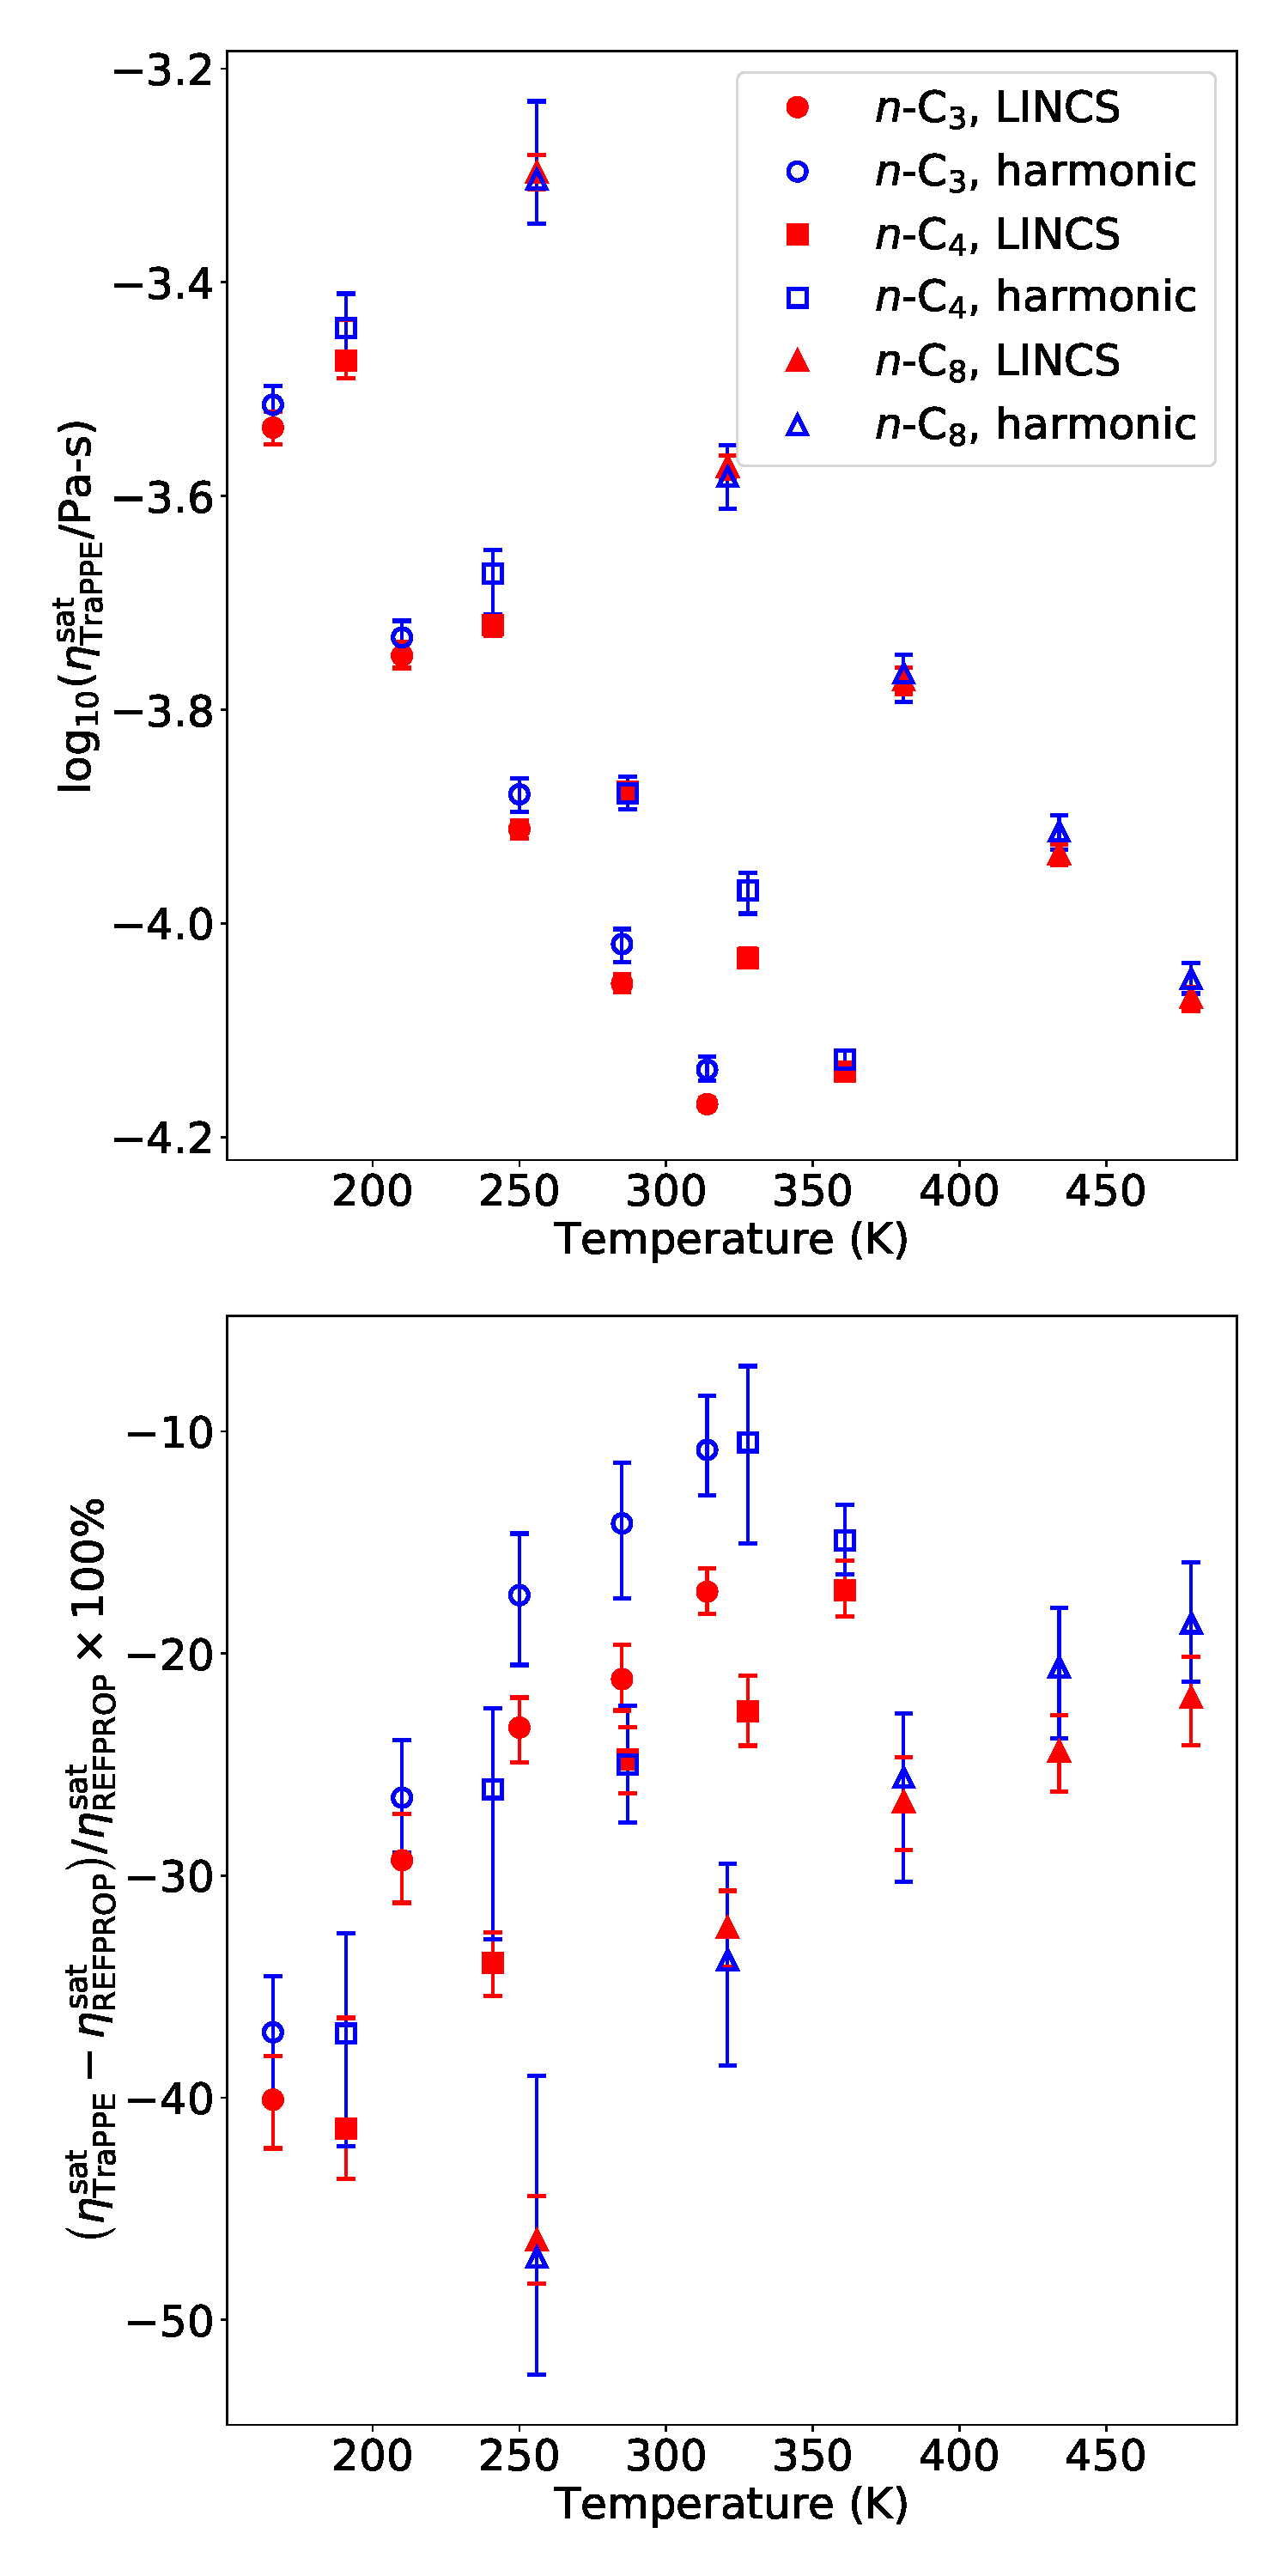
\includegraphics[width=3.2in]{nAlkanes_TraPPE_BondType.pdf}
		\caption{Fixed bond-lengths compared with an arbitrarily stiff harmonic bond potential. Simulations were performed using the TraPPE-UA force field. Colors/fill denote fixed or flexible bonds while symbol shape corresponds to different compounds.}
		\label{fig:fixed_flexible}
	\end{figure} 

%	To determine the impact, we perform simulations with two different values of $k_{\rm b}$, namely, BLANK (taken from reference BLANK) and BLANK (an arbitrarily large value). Figure \ref{fig:fixed_flexible} demonstrates that the difference between fixed and flexible bonds is negligible in certain cases, but for the larger force constant a systematic increase in viscosity is observed. 
%	
%	%Bootstrap re-sampling confirms that the LINCS and $k_{\rm b} = $ BLANK results are statistically indistinguishable, while the $k_{\rm b} = $ BLANK is statistically different.
%	
%	\begin{figure}[htb!]
%		\centering
%		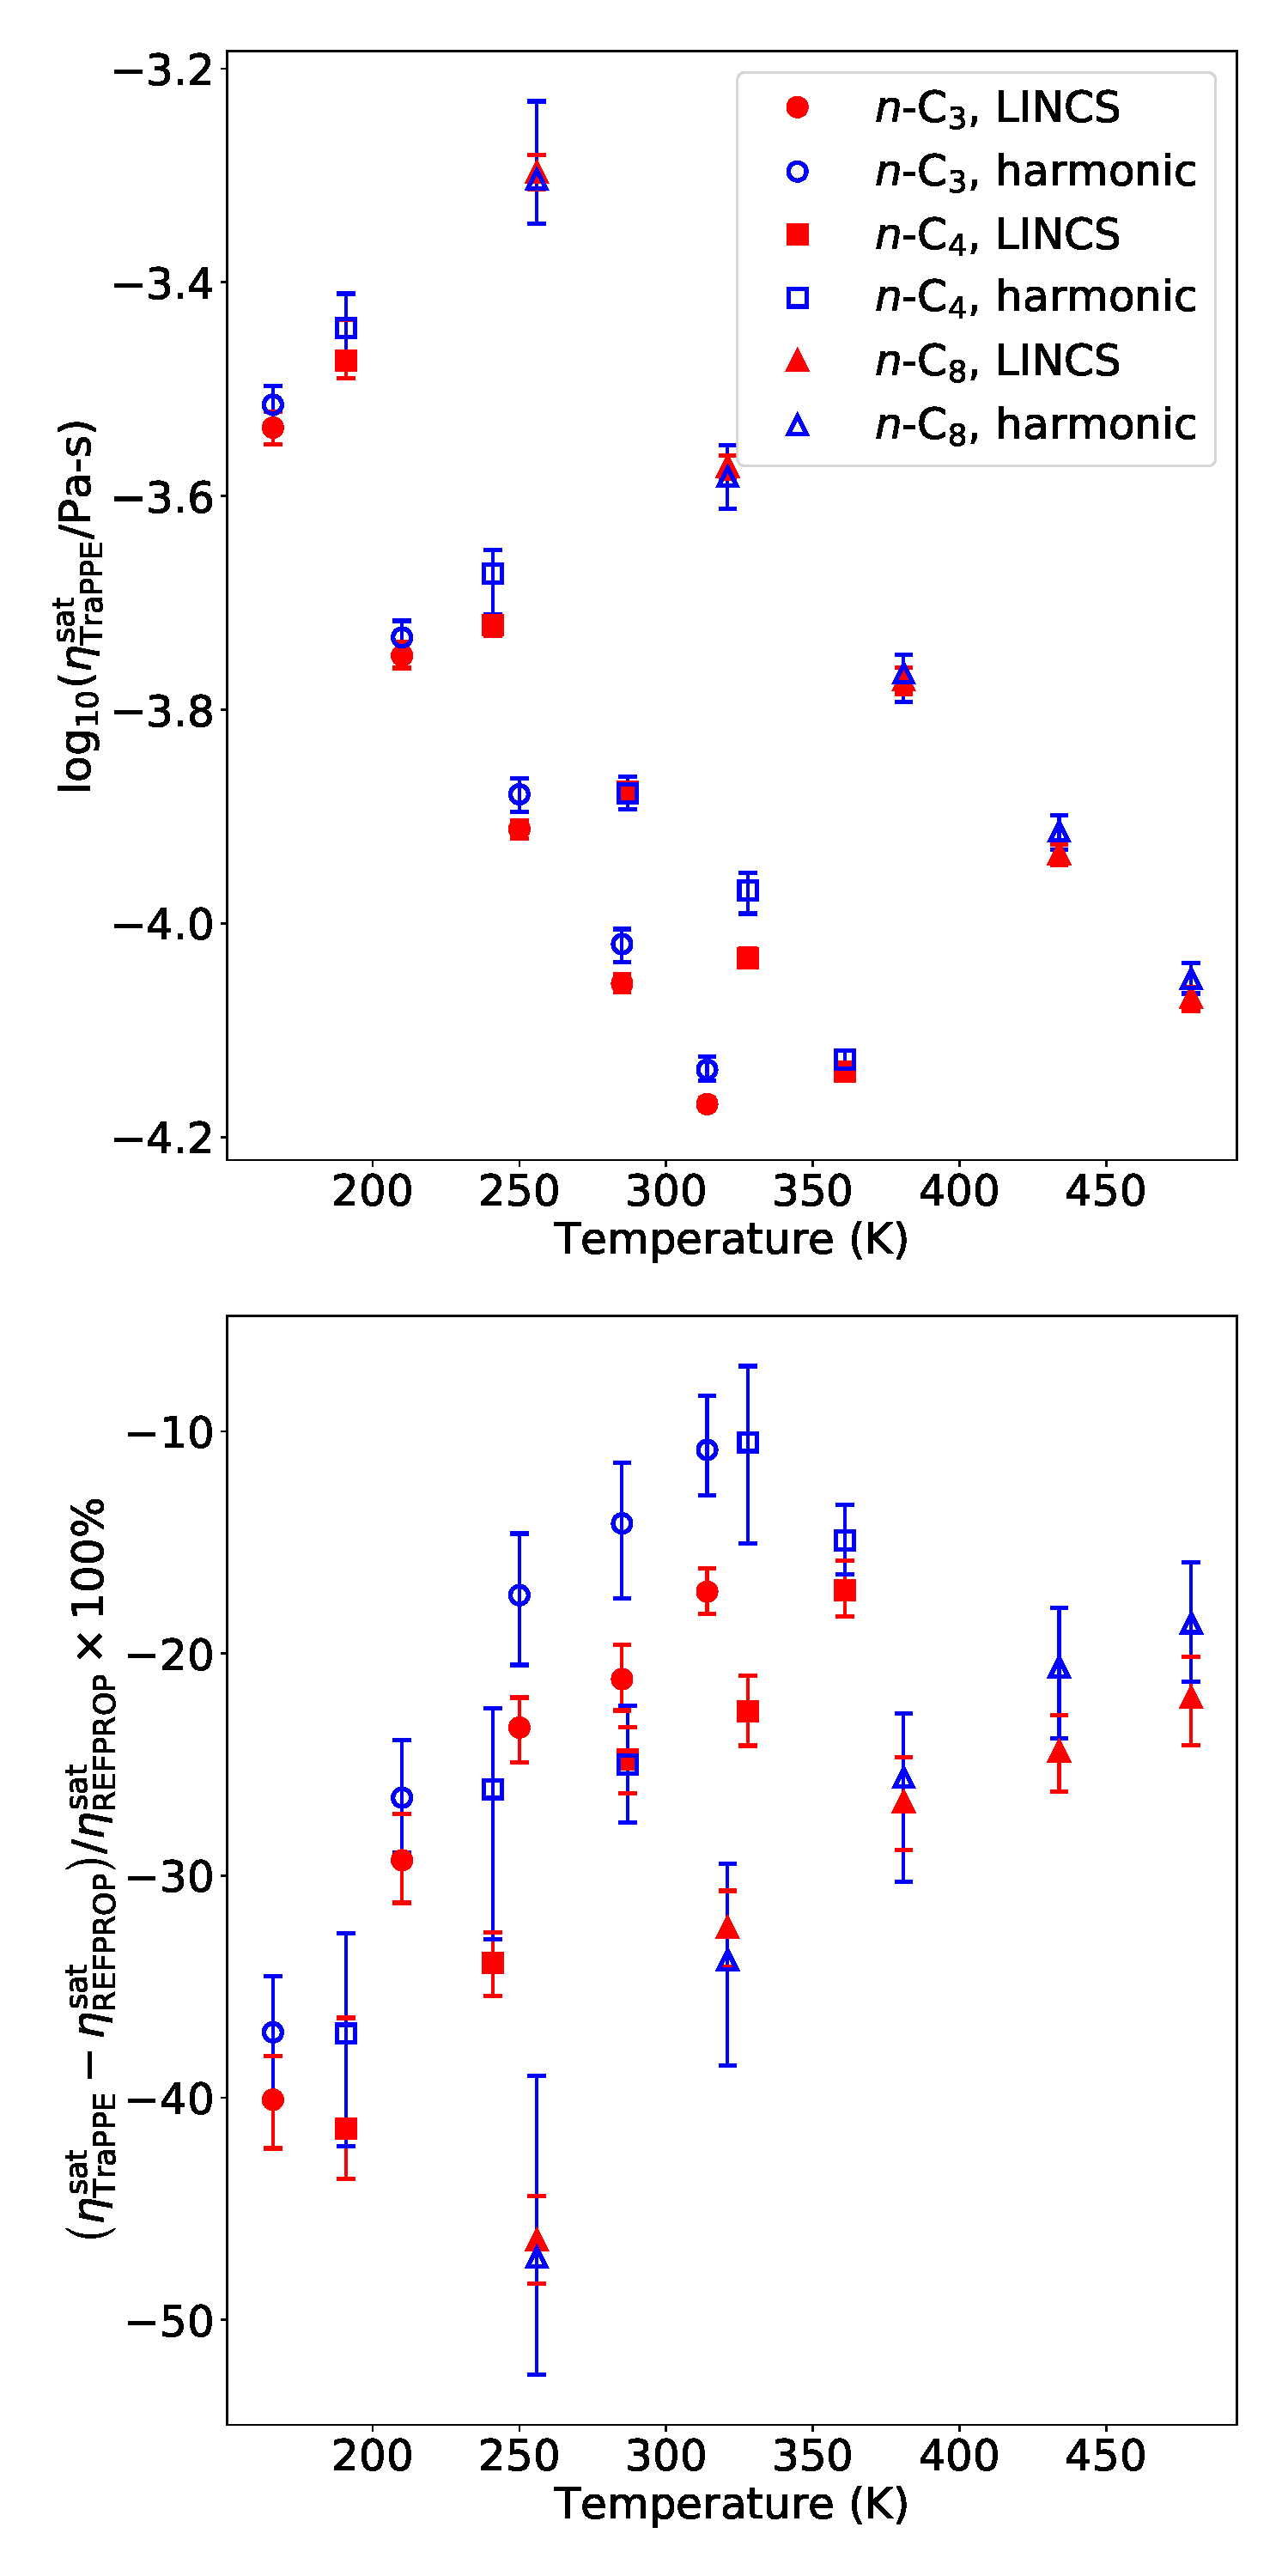
\includegraphics[width=3.2in]{nAlkanes_TraPPE_BondType.pdf}
%		\caption{Fixed bond-lengths compared with two different harmonic bond potentials.}
%		\label{fig:fixed_flexible}
%	\end{figure} 
	
%	\begin{enumerate}
%		\item Propane and n-butane with harmonic (arbirary bond constant) shows systematic increase
%	\end{enumerate}

    \clearpage
	\newpage
	
	\section{Green-Kubo analysis} \label{SI:GK_analysis}
	
	This section provides a detailed example of how we obtain estimates for $\eta$ and the corresponding uncertainty. The results depicted in Figures \ref{fig:autocorrelation} through \ref{fig:bootstraps} are for propane with the Potoff model and $T^{\rm sat} = 166$ K. Figure \ref{fig:autocorrelation} depicts a typical autocorrelation function (``enecorr.xvg'' file) obtained by executing the GROMACS ``energy --vis'' command. By default, GROMACS partitions the complete simulation into twelve evenly sized time blocks. Therefore, the autocorrelation function in Figure \ref{fig:autocorrelation} is the average of twelve different time origins. 
	
	GROMACS then performs a simple two-point trapezoidal integration of neighboring points to obtain the Green-Kubo integral. The Green-Kubo integral with respect to time is output in the ``visco.xvg'' file. Figure \ref{fig:replicates} presents the Green-Kubo integral from forty replicate simulations. Although a single replicate is often quite noisy at long times, the average of these replicates converges smoothly (see Figure \ref{fig:replicates}). 
	
	Figure \ref{fig:standard_deviation} shows that the fluctuations, or standard deviation, increases with time but is adequately modeled with $A t^{b}$. The line labeled ``cut-off'' in Figures \ref{fig:replicates} and \ref{fig:standard_deviation} is the time at which $\sigma_{\eta} \approx 0.4 \times \eta^\infty$. Data beyond this time are excluded from the fit of the double-exponential function. 
	
	Bootstrap re-sampling provides an estimate of the uncertainty. Figure \ref{fig:bootstraps} shows that, typically, the bootstrapped distribution is quite normal. The lines labeled ``bootstraps'' in Figure \ref{fig:replicates} are the lower and upper 95 \% confidence interval.
	
	\begin{figure}[htb!]
		\centering
		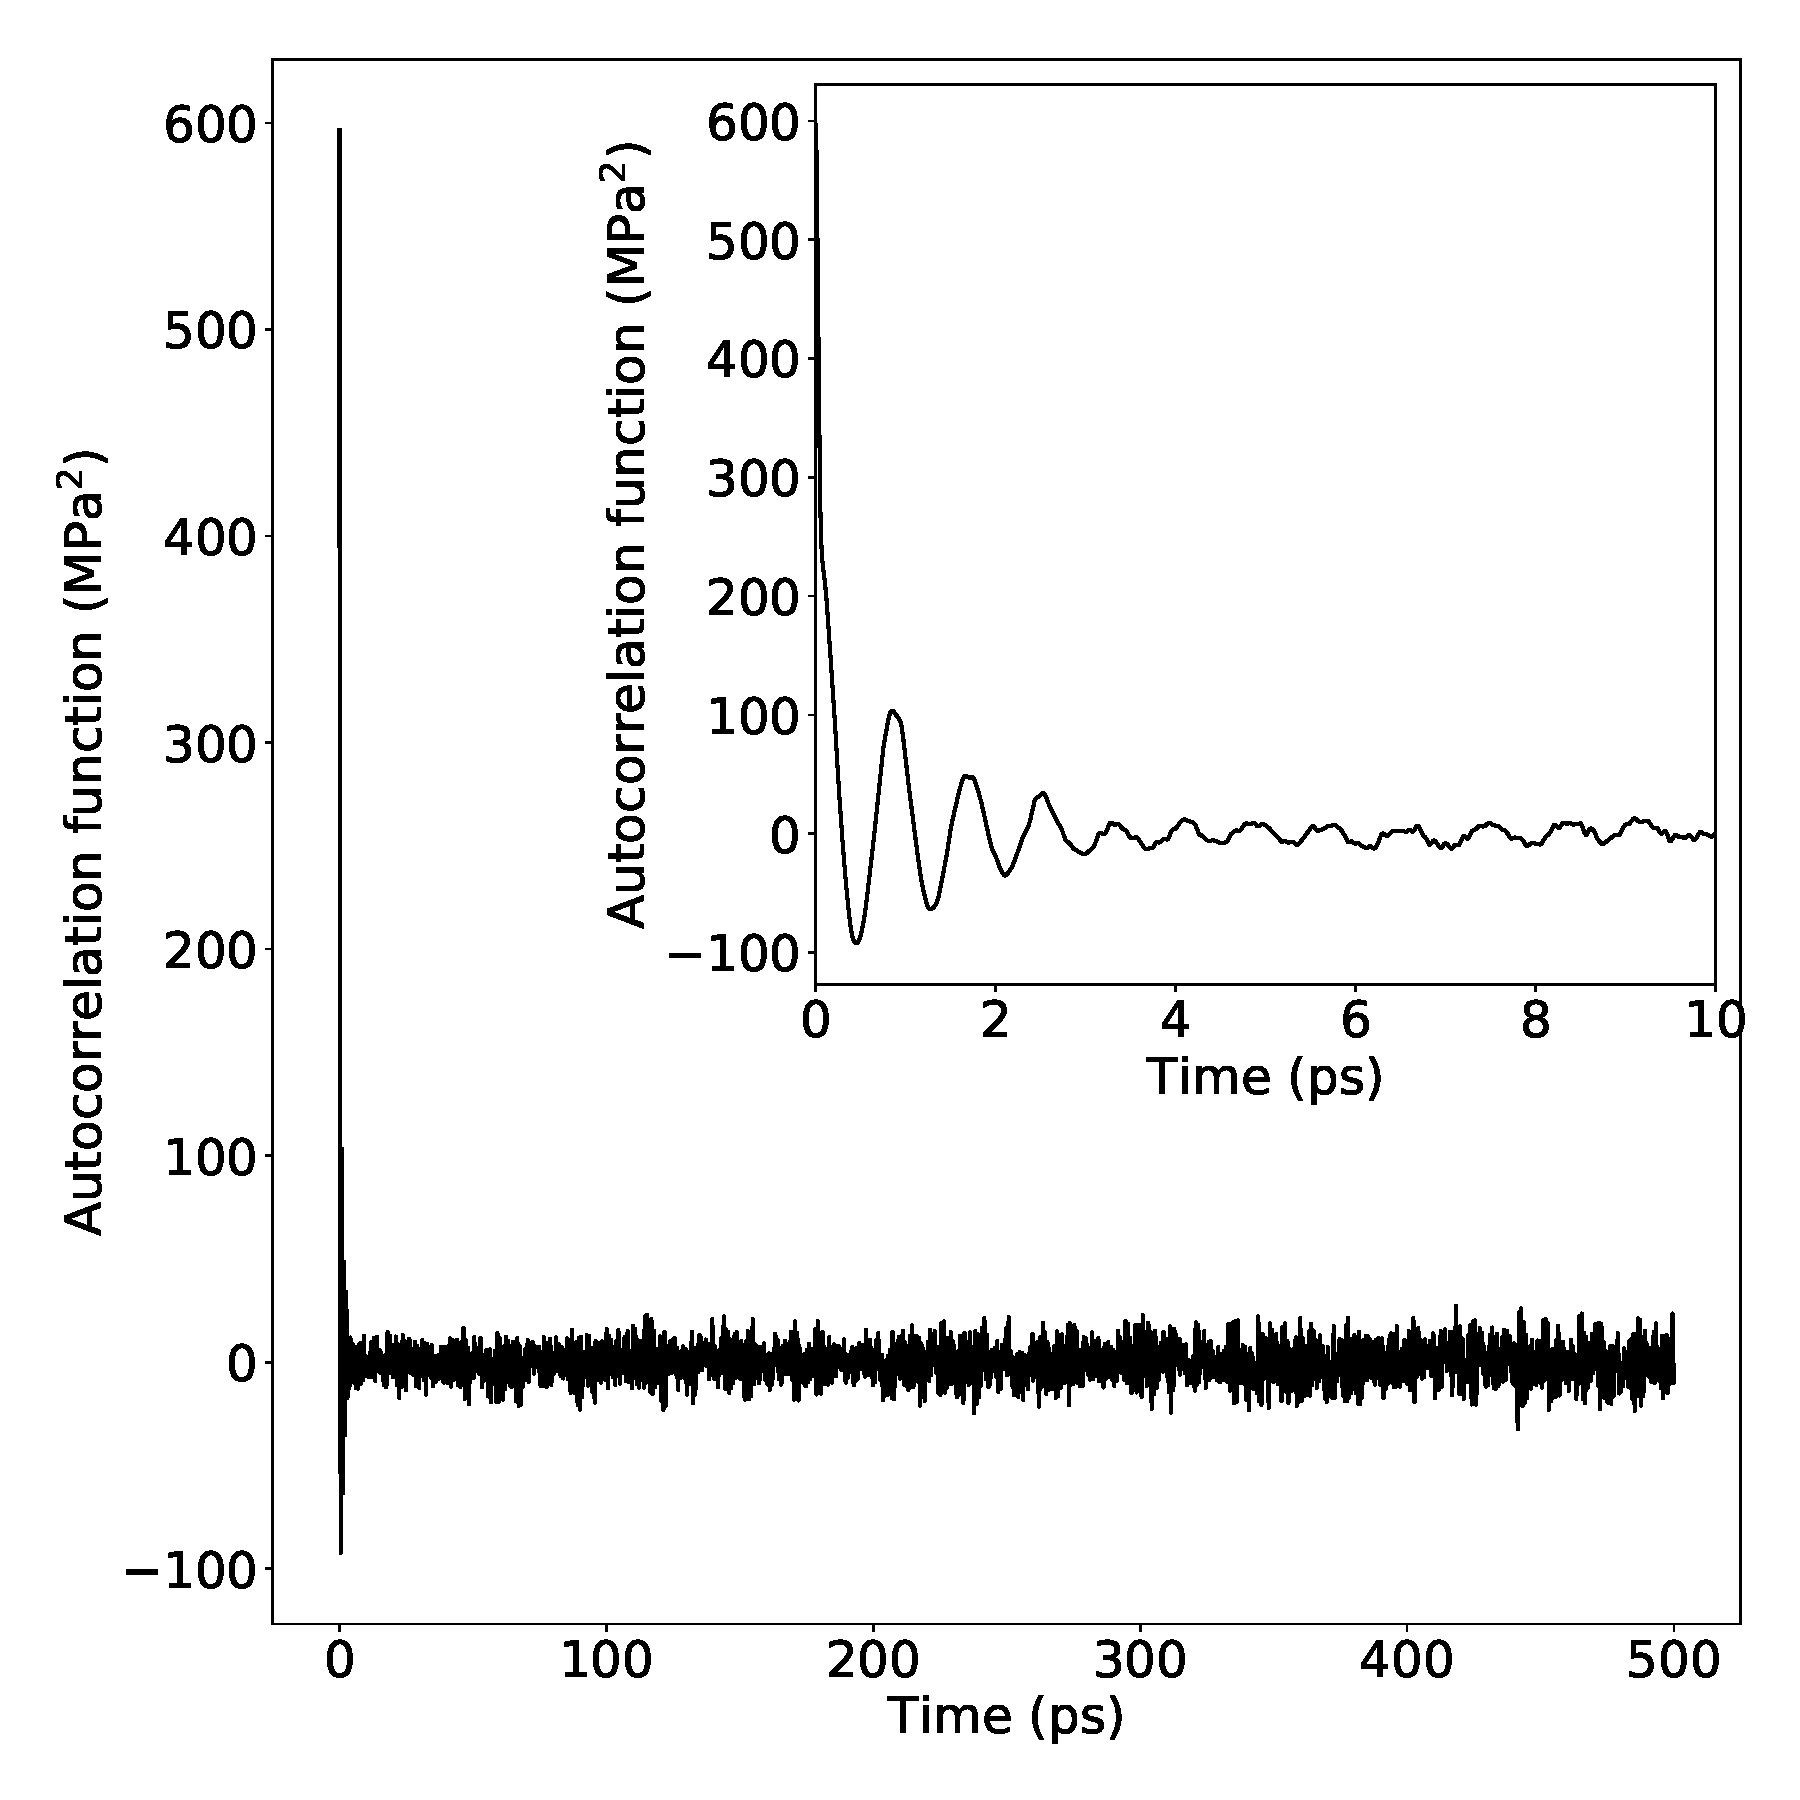
\includegraphics[width=3.2in]{autocorrelation_function.pdf}
		\caption{Autocorrelation function with respect to time.}
		\label{fig:autocorrelation}
	\end{figure} 

	\begin{figure}[htb!]
		\centering
		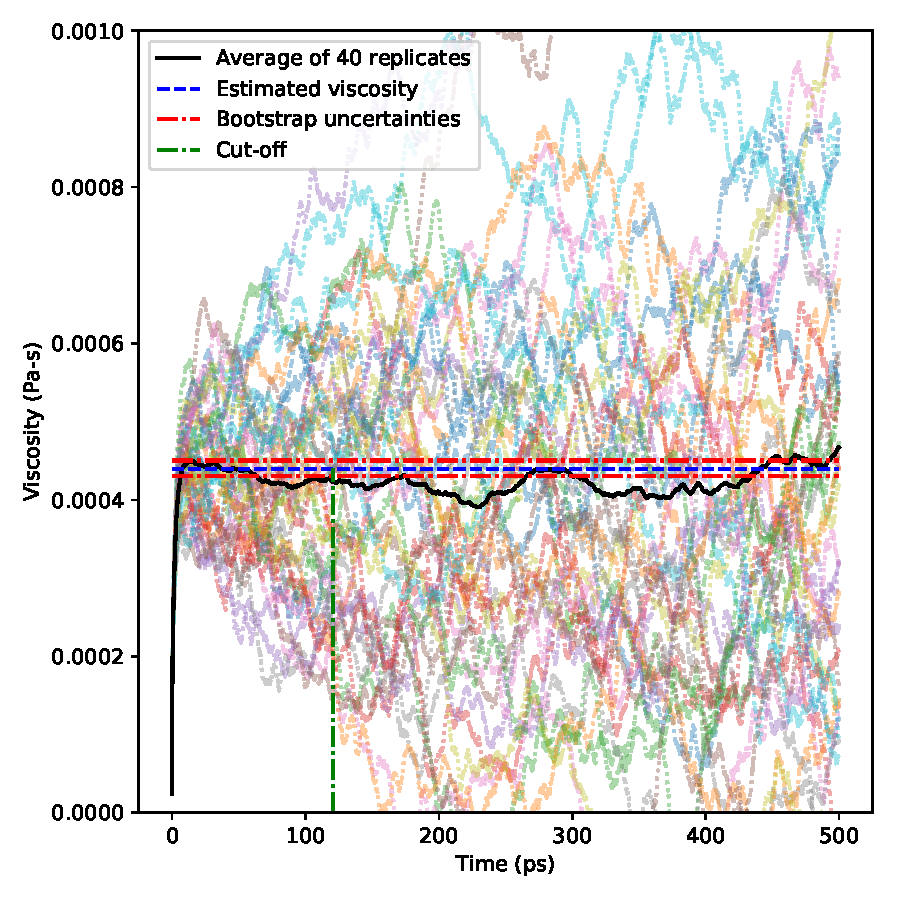
\includegraphics[width=3.2in]{GK_MCMC_all_rho0.pdf}
		\caption{Replicate simulations, average, fit to average, bootstrap uncertainties, and cut-off.}
		\label{fig:replicates}
	\end{figure} 

	\begin{figure}[htb!]
		\centering
		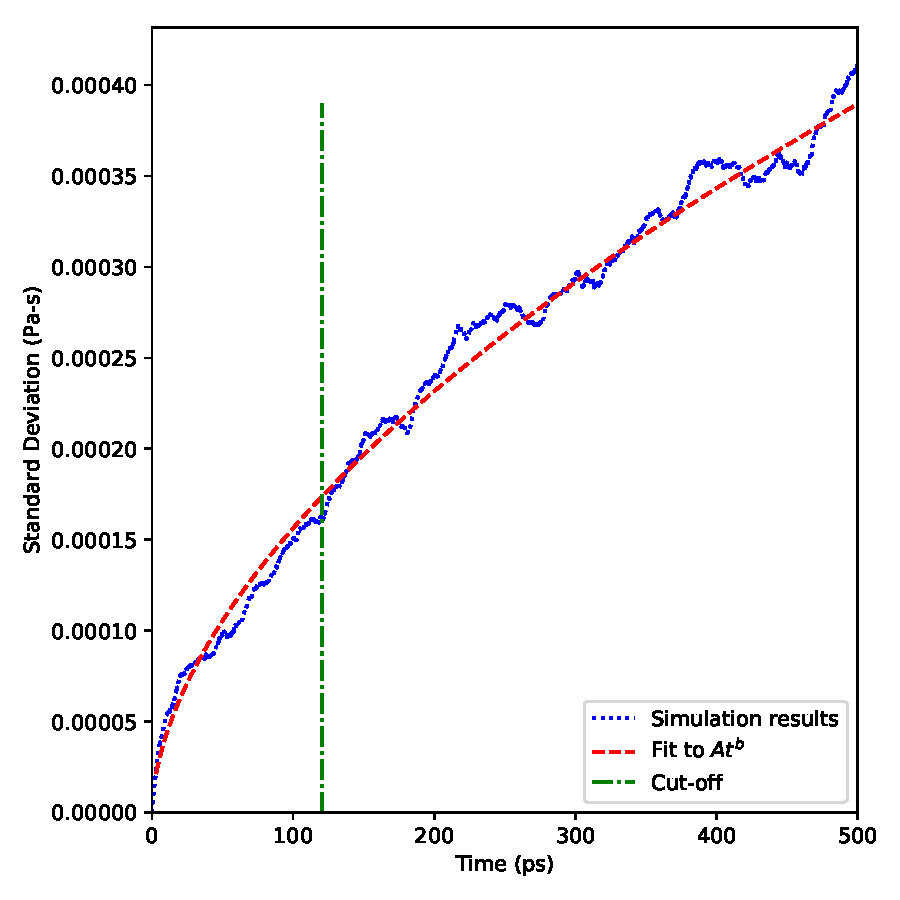
\includegraphics[width=3.2in]{sig_fit_rho0.pdf}
		\caption{Standard deviation of replicate simulations with respect to time.}
		\label{fig:standard_deviation}
	\end{figure} 

	\begin{figure}[htb!]
		\centering
		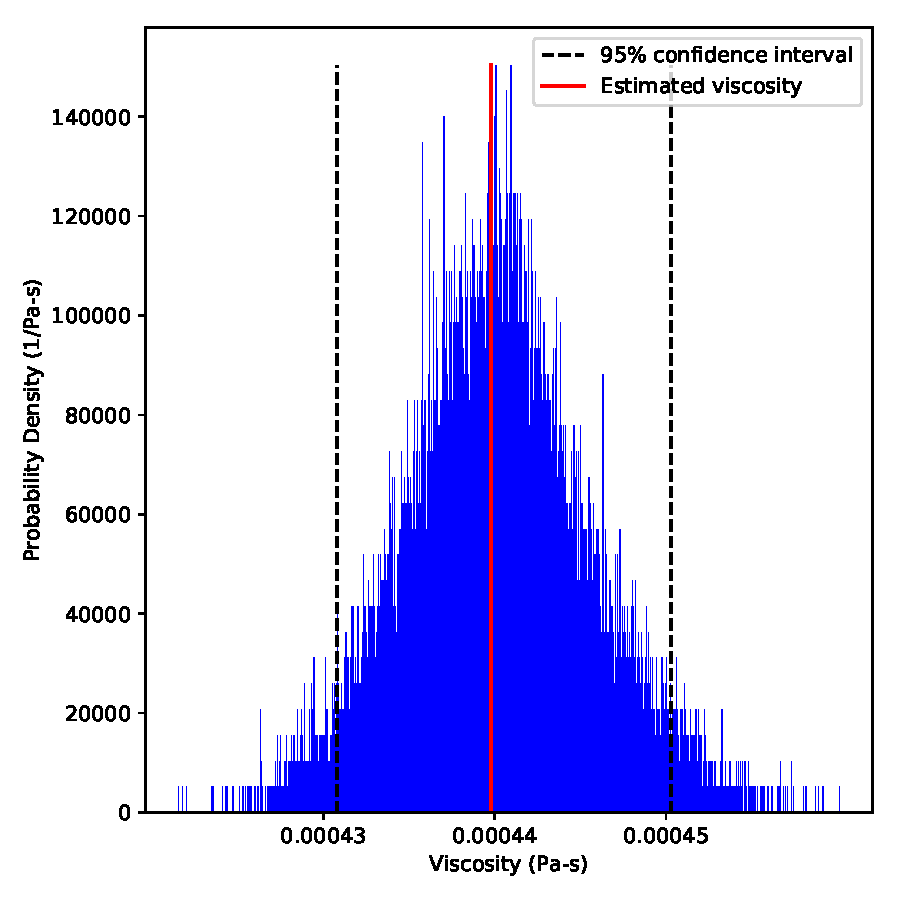
\includegraphics[width=3.2in]{GK_bootstraps_MCMC_rho0.pdf}
		\caption{Bootstrap distribution of $\eta$.}
		\label{fig:bootstraps}
	\end{figure} 

%	\begin{enumerate}
%		\item Raw data, i.e., multiple replicates with the average
%		\item Exclude low time data and have a heuristic for determining the cut-off time
%	\end{enumerate}
%	
%	Example analysis, i.e., bootstrap distribution, replicates
	
%	\subsection{MCMC?}

    \clearpage
	\newpage

	\section{Validation Runs} \label{Validation Runs}
	
	To validate our approach, we attempt to replicate viscosity estimates available on the NIST Standard Reference Simulation Website \cite{NIST_SRSW} for TraPPE-UA ethane as well as literature values for TraPPE-UA \textit{n}-octane \cite{Kioupis2000,Nieto2006}. Figures \ref{fig:validation_runs} and \ref{fig:validation_runs2} compare the ethane and \textit{n}-octane results, respectively. The \textit{n}-octane validation is somewhat more useful than the ethane validation for at least three reasons. First, \textit{n}-octane includes angle and torsional contributions that are absent in ethane. Second, the literature provides values for both rigid and flexible bonds. Third, the \textit{n}-octane results are at elevated pressures, which provides validation of our $NPT$ ensemble results. 
	
	% from this study with those from NIST and the literature, respectively.   
	
	\begin{figure}[htb!]
		\centering
		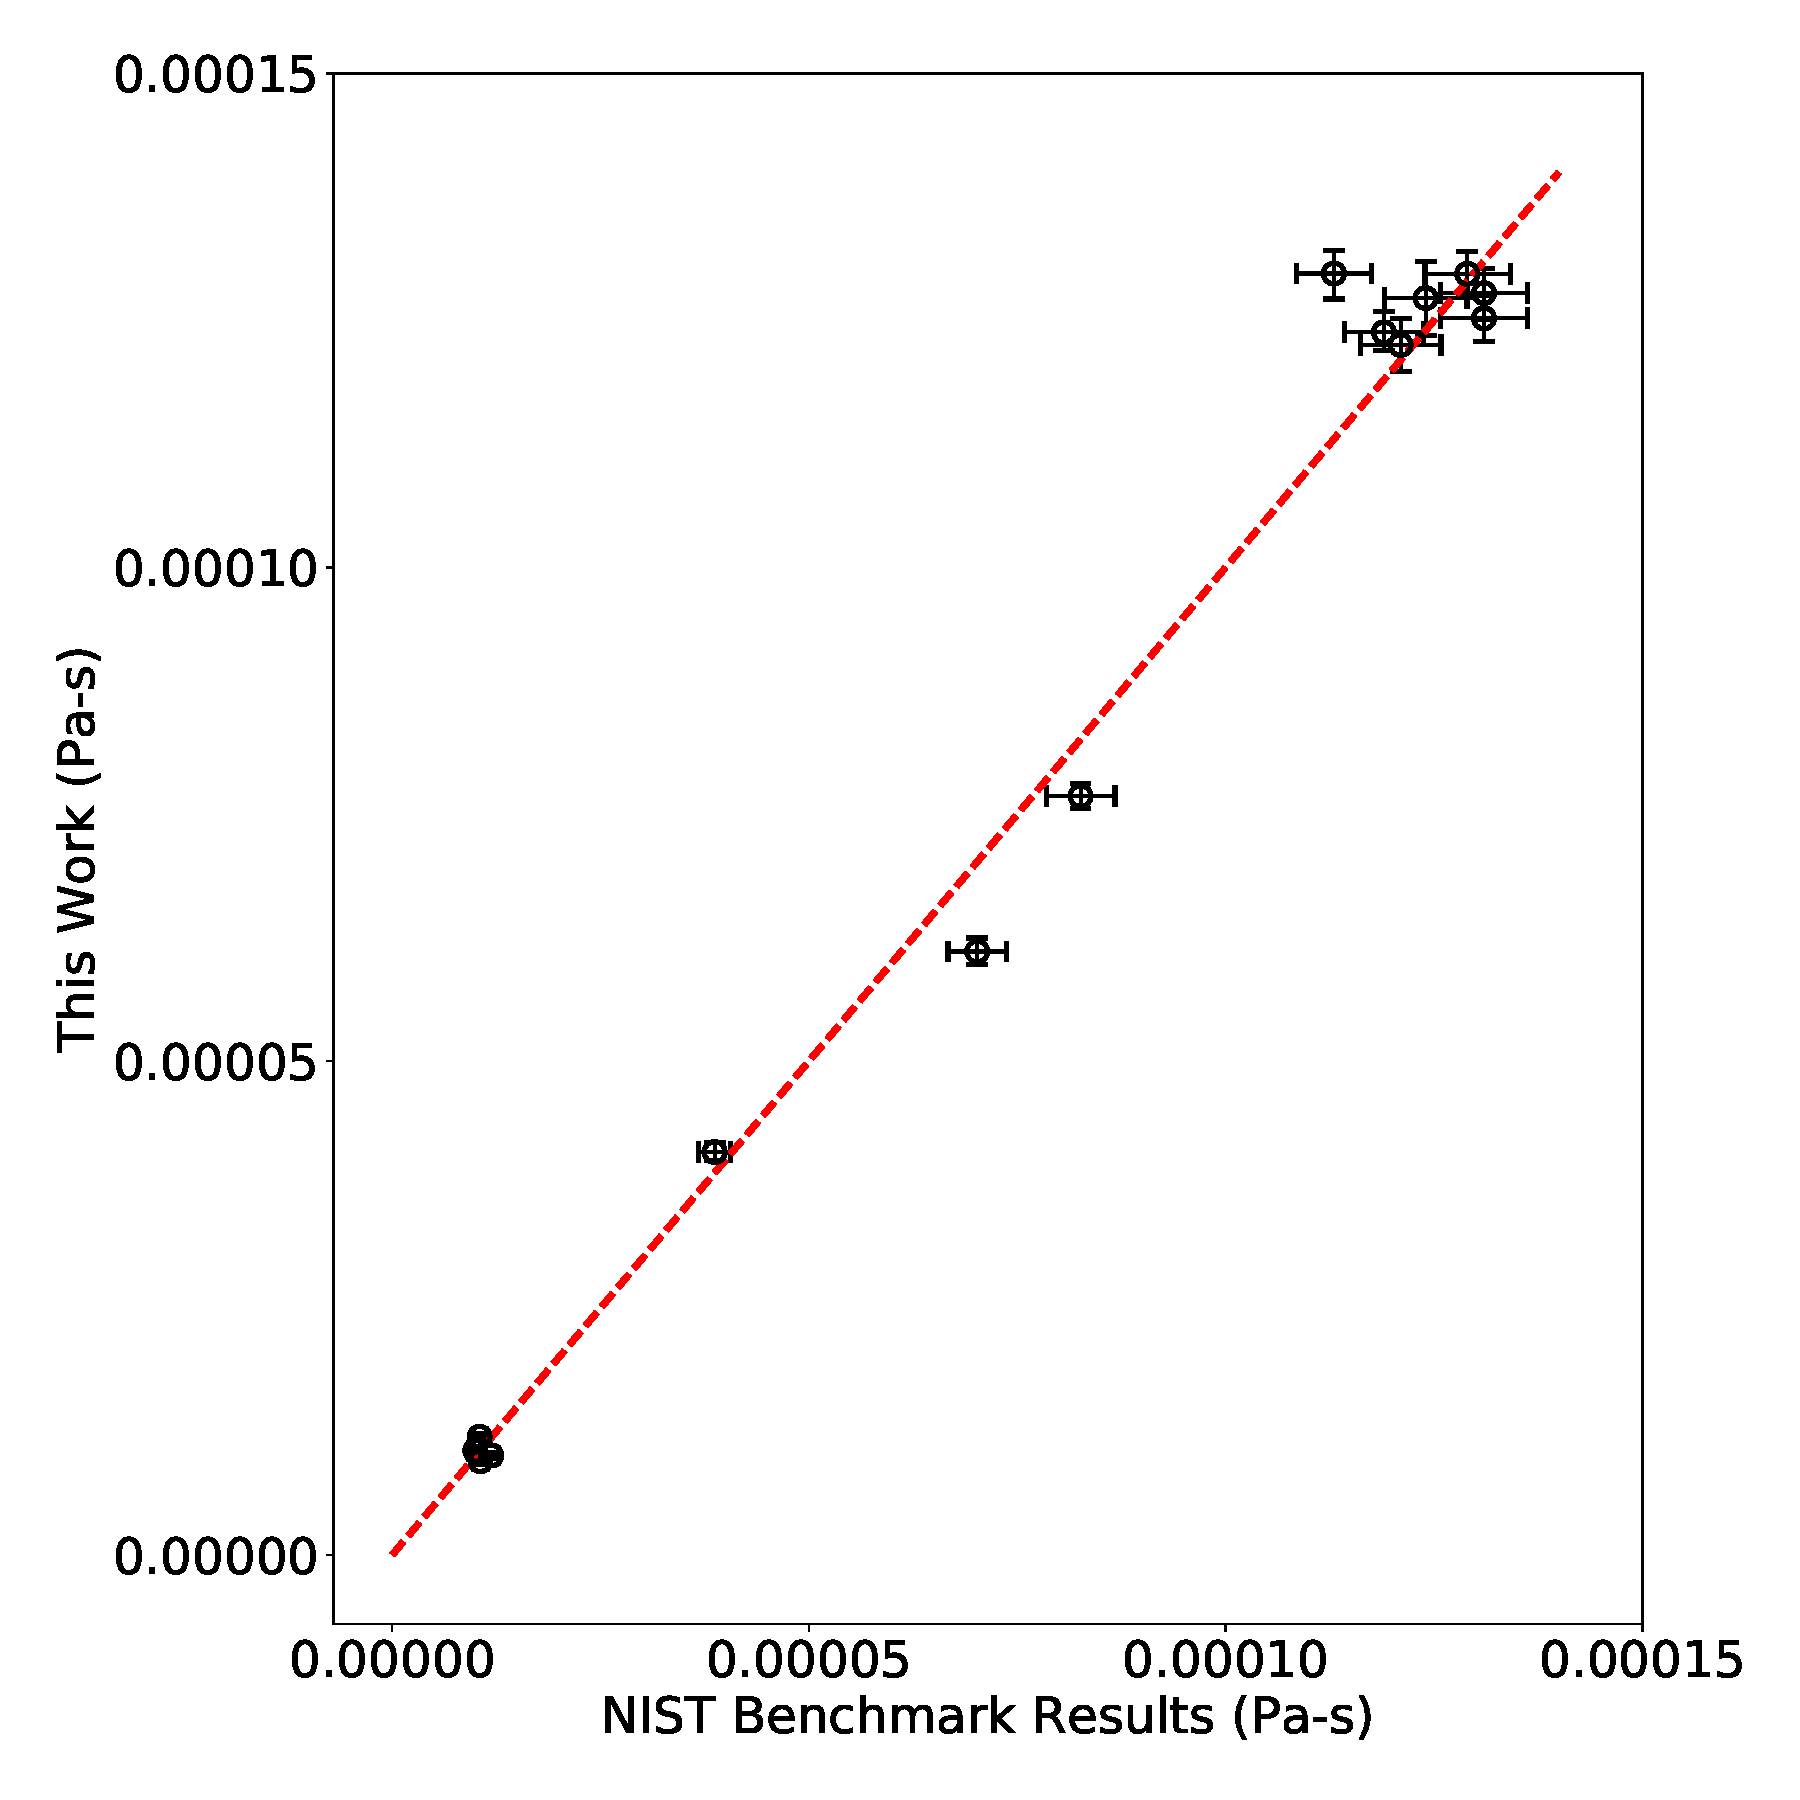
\includegraphics[width=3.2in]{NIST_ethane_TraPPE_validation.pdf}
		\caption{Comparison with NIST Standard Reference Simulation benchmark data for TraPPE ethane \cite{NIST_SRSW}. Red line corresponds to $x = y$, i.e., exact agreement between this work and the NIST values. A constant uncertainty of 4 \% is assumed for NIST values.}
		\label{fig:validation_runs}
	\end{figure} 
	
	Figure \ref{fig:validation_runs} demonstrates that our results are consistent with the NIST Reference Simulation Data at higher densities, with some discrepancies at lower densities. Note that the NIST Standard Reference Simulation benchmark data were obtained with the $NVE$ ensemble, while our simulations were performed with the $NVT$ ensemble at the average $T$ reported on the NIST website. Also, the NIST simulations used 500 molecules, 250 ps production time, and a 0.5 fs time-step.  
	
	\begin{figure}[htb!]
		\centering
		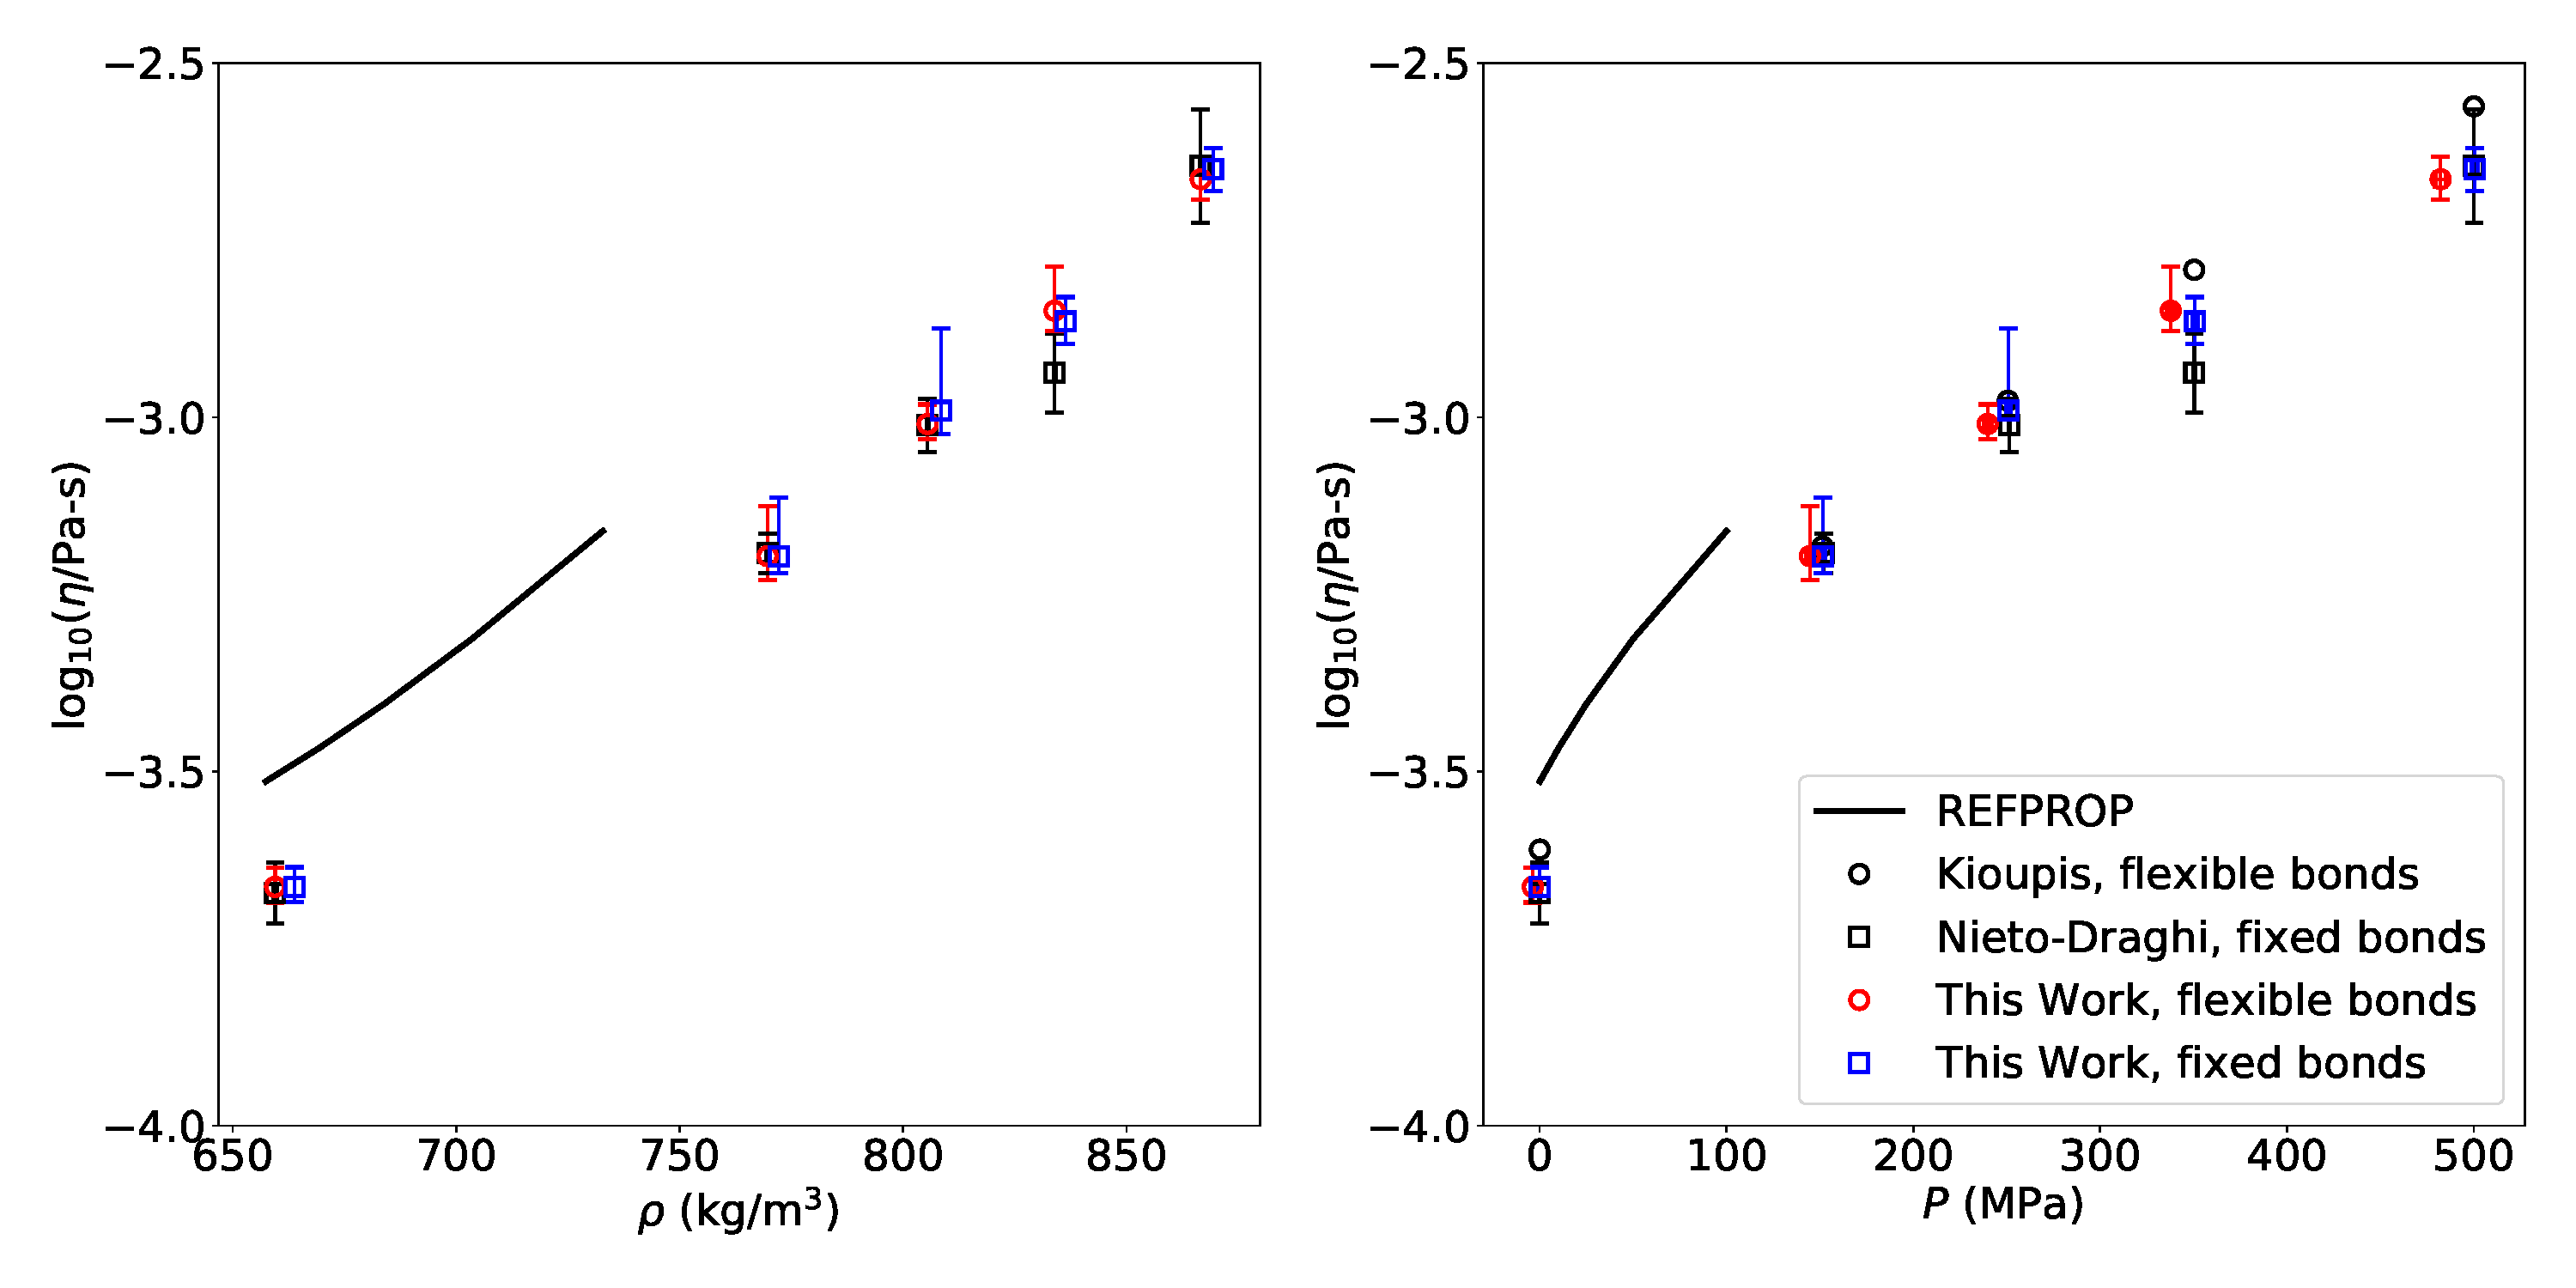
\includegraphics[width=6.4in]{validation_TraPPE_octane.pdf}
		\caption{Comparison with Kioupis \cite{Kioupis2000} and Nieto-Draghi \cite{Nieto2006} results for TraPPE \textit{n}-octane. Circle symbols were obtained with the same harmonic potential, while square symbols denote fixed bond-lengths.}
		\label{fig:validation_runs2}
	\end{figure}
	
	Figure \ref{fig:validation_runs2} demonstrates that our results agree with the literature values for TraPPE \textit{n}-octane at high pressures. Note that our flexible bond results utilize the same harmonic potential as Reference \citenum{Kioupis2000} ($k_{\rm b}/k_{\rm B} = 45.29$ K/pm$^2$, value actually reported in Reference \citenum{Kioupis1999}). Thus, by comparing the circular points, there is an apparent positive bias between the Reference \citenum{Kioupis2000} values and those from this work. We note that Reference \citenum{Kioupis2000} utilizes NEMD simulations, where extrapolation to zero shear is necessary. From this result, we suggest that the extrapolation tends to over estimate the true viscosity. Furthermore, by comparing the fixed and flexible bond results we see a small shift towards higher viscosities for the harmonic potential. This is investigated further in Section \ref{fixed flexible}.
	
	%Thus, the comparison between literature and ``this work'' should only be made for circle symbols and square symbols. By comparing the harmonic potential results, there is an apparent positive bias between the Reference \citenum{Kioupis2000} values and those from this work. We note that Reference \citenum{Kioupis2000} utilizes NEMD simulations, where extrapolation to zero shear is necessary. From this result, we suggest that the extrapolation tends to over estimate the true viscosity.
	
	% while Reference \citenum{Nieto2006} performed EMD simulations with fixed bond-lengths.
	
	It is important to note that Reference \citenum{Nieto2006} utilizes a 1.0 nm cut-off, whereas we use a 1.4 nm cut-off. As demonstrated in Section \ref{Discussion/Limitations} of the manuscript, the results for a 1.0 nm and 1.4 nm cut-off can become significant for larger molecules. However, due to the good agreement between our values and those from Reference \citenum{Nieto2006}, the 1.0 nm cut-off appears to be sufficient for \textit{n}-octane at elevated pressures. It is also worth noting that Reference \citenum{Nieto2006} performed 10 to 20 ns simulations, while our simulation production time was only 1 ns.
	
	Note that there appears to be a slight bias towards smaller box-sizes (higher $\rho$) for a given pressure when comparing the fixed bond-lengths from this work with the values of Reference \citenum{Nieto2006}. Also, small discrepancies exist between the state points reported in Reference \citenum{Kioupis2000} and Reference \citenum{Nieto2006}. This should not impact our validation, but it is somewhat curious. 
	
	%	
	%	\begin{enumerate}
	%		\item Ethane NIST
	%		\item n-Octane Literature
	%	\end{enumerate}

    \clearpage
    
    \section{RDF in real units} \label{SI:RDF_real}
    
    Figure \ref{fig:RDF_comparison_CH3_real} presents the same data as Figure \ref{fig:RDF_comparison_CH3} of the main text, but with the non-bonded distance in real units.
    
    \begin{figure}[htb!]
    	\centering
    	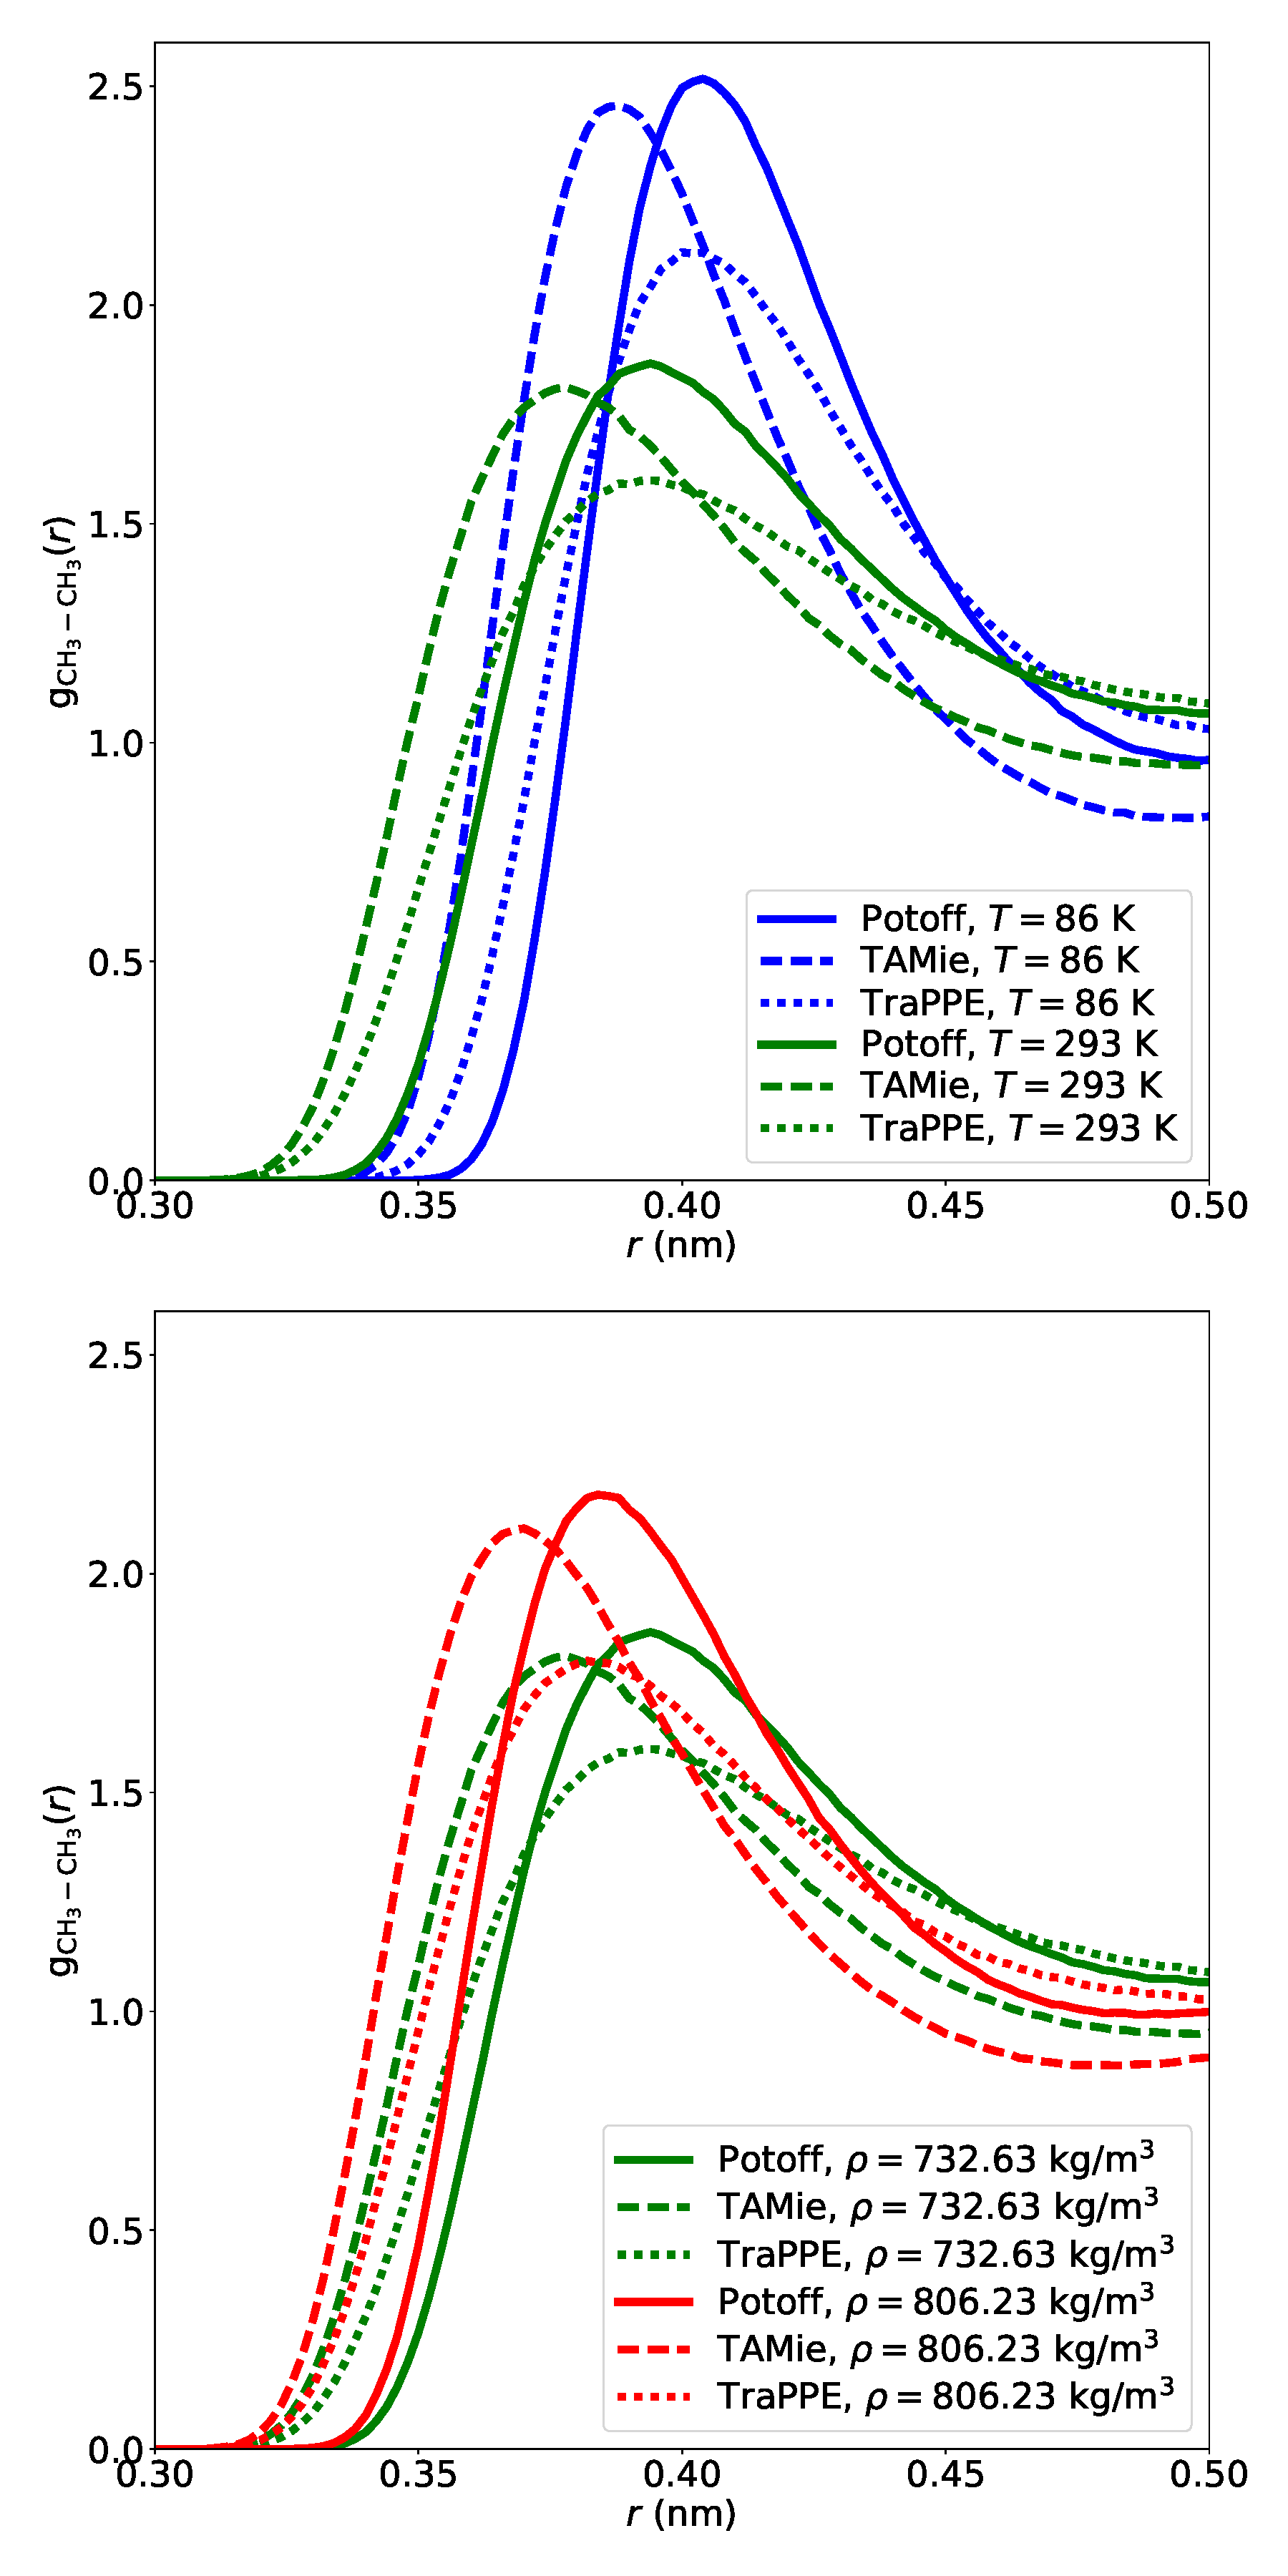
\includegraphics[width=3.2in]{RDF_comparison_CH3_real_units.pdf}
    	\caption{Comparison of radial distribution functions for CH$_3$-CH$_3$ interactions $(g_{\rm CH_3-CH_3}(r))$ with $r$ in real units. The top panel compares two different temperatures along the triple point isochore. The bottom panel compares two different densities along the 293 K isotherm. Colors correspond to different state points while line styles denote different force fields.}
    	\label{fig:RDF_comparison_CH3_real}
    \end{figure}
    
    \clearpage
    \newpage

	\section{Tabulated values} \label{SI:Tabulated}
	
	\begin{table}[H]
		\caption{Saturated liquid viscosity values for ethane.}
		\begin{center}
			\begin{tabular}{|c|c|c|c|c|c|c|}
				\hline
				&                                       & Potoff            & TAMie             & TraPPE 	& AUA4	& TraPPE-2            \\ \hline
				$T^{\rm sat}$ {[}K{]} & $\rho^{\rm sat}_{\rm liq}$ [kg/m$^3$] & $\eta_{\rm liq}^{\rm sat}$ {[}mPa-s{]} & $\eta_{\rm liq}^{\rm sat}$ {[}mPa-s{]} & $\eta_{\rm liq}^{\rm sat}$ {[}mPa-s{]} & $\eta_{\rm liq}^{\rm sat}$ {[}mPa-s{]} & $\eta_{\rm liq}^{\rm sat}$ {[}mPa-s{]} \\ \hline
				137 & 600.04 & 0.516$_{0.024}$   & 0.389$_{0.013}$   & 0.313$_{0.014}$   & 0.321$_{0.011}$   & 0.2981$_{8.5 \rm E-3}$ \\ \hline
				174 & 557.16 & 0.2338$_{4.8 \rm E-3}$ & 0.2046$_{4.0 \rm E-3}$ & 0.1714$_{3.7 \rm E-3}$ & 0.1741$_{4.1 \rm E-3}$ & 0.1773$_{3.3 \rm E-3}$ \\ \hline
				207 & 514.33 & 0.1499$_{3.3 \rm E-3}$ & 0.1360$_{3.0 \rm E-3}$ & 0.1123$_{2.5 \rm E-3}$ & 0.1185$_{3.6 \rm E-3}$ & 0.1204$_{2.1 \rm E-3}$ \\ \hline
				236 & 471.45 & 0.0991$_{2.4 \rm E-3}$ & 0.0976$_{2.1 \rm E-3}$ & 0.0844$_{1.8 \rm E-3}$ & 0.0837$_{2.2 \rm E-3}$ & 0.0876$_{1.2 \rm E-3}$ \\ \hline
				260 & 428.60 & 0.0732$_{1.3 \rm E-3}$ & 0.0709$_{1.3 \rm E-3}$ & 0.0623$_{1.1 \rm E-3}$ & 0.0629$_{1.9 \rm E-3}$ & 0.0661$_{1.3 \rm E-3}$ \\ \hline
			\end{tabular}
		\end{center}
	\end{table}

	\begin{table}[H]
		\caption{Saturated liquid viscosity values for propane.}
		\begin{center}
			\begin{tabular}{|c|c|c|c|c|}
				\hline
				&                                       & Potoff            & TAMie             & TraPPE            \\ \hline
				$T^{\rm sat}$ {[}K{]} & $\rho^{\rm sat}_{\rm liq}$ [kg/m$^3$] & $\eta_{\rm liq}^{\rm sat}$ {[}mPa-s{]} & $\eta_{\rm liq}^{\rm sat}$ {[}mPa-s{]} & $\eta_{\rm liq}^{\rm sat}$ {[}mPa-s{]} \\ \hline
				86 & 732.21 & 10.7$_{1.5}$      & 5.31$_{0.40}$     & 2.47$_{0.16}$     \\ \hline
				90 & 728.03 & 8.34$_{0.96}$     & 4.42$_{0.22}$     & 2.01$_{0.12}$     \\ \hline
				100  & 717.71 & 3.56$_{0.22}$     & 2.53$_{0.18}$     & 1.243$_{0.049}$   \\ \hline
				110  & 707.53 & 2.17$_{0.12}$     & 1.500$_{0.060}$   & 0.898$_{0.039}$   \\ \hline
				130  & 687.26 & 1.003$_{0.033}$   & 0.844$_{0.026}$   & 0.517$_{0.013}$   \\ \hline
				166  & 651.14 & 0.439$_{0.011}$   & 0.389$_{0.013}$   & 0.2967$_{8.3 \rm E-3}$ \\ \hline
				210  & 604.63 & 0.2482$_{9.4 \rm E-3}$ & 0.2361$_{9.5 \rm E-3}$ & 0.1800$_{4.0 \rm E-3}$ \\ \hline
				250  & 558.12 & 0.1513$_{4.9 \rm E-3}$ & 0.1498$_{5.3 \rm E-3}$ & 0.1234$_{3.1 \rm E-3}$ \\ \hline
				285  & 511.61 & 0.1040$_{3.2 \rm E-3}$ & 0.1055$_{3.8 \rm E-3}$ & 0.0874$_{1.5 \rm E-3}$ \\ \hline
				314  & 465.10 & 0.0761$_{1.9 \rm E-3}$ & 0.0797$_{2.6 \rm E-3}$ & 0.0676$_{1.2 \rm E-3}$ \\ \hline
			\end{tabular}
		\end{center}
	\end{table}
	
	\begin{table}[H]
		\caption{Saturated liquid viscosity values for \textit{n}-butane.}
		\begin{center}
			\begin{tabular}{|c|c|c|c|c|}
				\hline
				&                                       & Potoff            & TAMie             & TraPPE            \\ \hline
				$T^{\rm sat}$ {[}K{]} & $\rho^{\rm sat}_{\rm liq}$ [kg/m$^3$] & $\eta_{\rm liq}^{\rm sat}$ {[}mPa-s{]} & $\eta_{\rm liq}^{\rm sat}$ {[}mPa-s{]} & $\eta_{\rm liq}^{\rm sat}$ {[}mPa-s{]} \\ \hline
				191 & 341.27 & 0.551$_{0.019}$   & 0.604$_{0.030}$   & 0.336$_{0.029}$   \\ \hline
				241 & 316.89 & 0.286$_{0.013}$   & 0.2664$_{6.2 \rm E-3}$ & 0.1900$_{4.3 \rm E-3}$ \\ \hline
				287 & 292.52 & 0.1690$_{3.6 \rm E-3}$ & 0.1640$_{3.7 \rm E-3}$ & 0.1327$_{2.7 \rm E-3}$ \\ \hline
				328 & 268.14 & 0.1147$_{2.2 \rm E-3}$ & 0.1168$_{1.8 \rm E-3}$ & 0.0928$_{2.0 \rm E-3}$ \\ \hline
				361 & 243.76 & 0.0858$_{1.6 \rm E-3}$ & 0.0849$_{2.1 \rm E-3}$ & 0.0726$_{1.2 \rm E-3}$ \\ \hline
			\end{tabular}
		\end{center}
	\end{table}
	
	\begin{table}[H]
		\caption{Saturated liquid viscosity values for \textit{n}-octane.}
		\begin{center}
			\begin{tabular}{|c|c|c|c|c|}
				\hline
				&                                       & Potoff            & TAMie             & TraPPE            \\ \hline
				$T^{\rm sat}$ {[}K{]} & $\rho^{\rm sat}_{\rm liq}$ [kg/m$^3$] & $\eta_{\rm liq}^{\rm sat}$ {[}mPa-s{]} & $\eta_{\rm liq}^{\rm sat}$ {[}mPa-s{]} & $\eta_{\rm liq}^{\rm sat}$ {[}mPa-s{]} \\ \hline
				256 & 732.07 & 0.830$_{0.041}$   & 0.870$_{0.029}$   & 0.504$_{0.019}$   \\ \hline
				321 & 679.78 & 0.373$_{0.011}$   & 0.373$_{0.010}$   & 0.2675$_{7.0 \rm E-3}$ \\ \hline
				381 & 627.49 & 0.2231$_{0.010}$  & 0.2378$_{5.9 \rm E-3}$ & 0.1689$_{4.9 \rm E-3}$ \\ \hline
				434 & 575.20 & 0.1385$_{5.9 \rm E-3}$ & 0.1416$_{3.5 \rm E-3}$ & 0.1161$_{2.8 \rm E-3}$ \\ \hline
				479 & 522.91 & 0.1053$_{4.7 \rm E-3}$ & 0.1024$_{7.4 \rm E-3}$ & 0.0851$_{2.4 \rm E-3}$ \\ \hline
			\end{tabular}
		\end{center}
	\end{table}
	
	\begin{table}[H]
		\caption{Saturated liquid viscosity values for \textit{n}-dodecane.}
		\begin{center}
			\begin{tabular}{|c|c|c|c|c|}
				\hline
				&                                       & Potoff            & TAMie             & TraPPE            \\ \hline
				$T^{\rm sat}$ {[}K{]} & $\rho^{\rm sat}_{\rm liq}$ [kg/m$^3$] & $\eta_{\rm liq}^{\rm sat}$ {[}mPa-s{]} & $\eta_{\rm liq}^{\rm sat}$ {[}mPa-s{]} & $\eta_{\rm liq}^{\rm sat}$ {[}mPa-s{]} \\ \hline
				296 & 747.27 & 1.056$_{0.065}$   & 1.009$_{0.048}$   & 0.691$_{0.049}$   \\ \hline
				362 & 698.31 & 0.487$_{0.024}$   & 0.487$_{0.014}$   & 0.349$_{0.014}$   \\ \hline
				427 & 647.90 & 0.2768$_{8.1 \rm E-3}$ & 0.2868$_{8.7 \rm E-3}$ & 0.2180$_{7.0 \rm E-3}$ \\ \hline
				493 & 590.68 & 0.1799$_{5.5 \rm E-3}$ & 0.1780$_{7.0 \rm E-3}$ & 0.1442$_{5.0 \rm E-3}$ \\ \hline
				559 & 520.47 & 0.1066$_{2.8 \rm E-3}$ & 0.1114$_{4.3 \rm E-3}$ & 0.0937$_{2.1 \rm E-3}$ \\ \hline
			\end{tabular}
		\end{center}
	\end{table}
	
	\begin{table}[H]
		\caption{Saturated liquid viscosity values for \textit{n}-hexadecane.}
		\begin{center}
			\begin{tabular}{|c|c|c|c|c|}
				\hline
				&                                       & Potoff            & TAMie             & TraPPE            \\ \hline
				$T^{\rm sat}$ {[}K{]} & $\rho^{\rm sat}_{\rm liq}$ [kg/m$^3$] & $\eta_{\rm liq}^{\rm sat}$ {[}mPa-s{]} & $\eta_{\rm liq}^{\rm sat}$ {[}mPa-s{]} & $\eta_{\rm liq}^{\rm sat}$ {[}mPa-s{]} \\ \hline
				325 & 751.26 & 1.225$_{0.092}$   & 1.217$_{0.094}$   & 0.794$_{0.047}$   \\ \hline
				397 & 700.84 & 0.572$_{0.027}$   & 0.568$_{0.023}$   & 0.439$_{0.017}$   \\ \hline
				469 & 648.85 & 0.364$_{0.025}$   & 0.329$_{0.017}$   & 0.264$_{0.010}$   \\ \hline
				541 & 592.22 & 0.1956$_{6.4 \rm E-3}$ & 0.1917$_{6.9 \rm E-3}$ & 0.1752$_{6.1 \rm E-3}$ \\ \hline
				613 & 524.45 & 0.1296$_{3.5 \rm E-3}$ & 0.1249$_{4.0 \rm E-3}$ & 0.1114$_{4.7 \rm E-3}$ \\ \hline
			\end{tabular}
		\end{center}
	\end{table}
	
	\begin{table}[H]
		\caption{Saturated liquid viscosity values for \textit{n}-docosane.}
		\begin{center}
			\begin{tabular}{|c|c|c|c|c|}
				\hline
				&                                       & Potoff            & TAMie             & TraPPE            \\ \hline
				$T^{\rm sat}$ {[}K{]} & $\rho^{\rm sat}_{\rm liq}$ [kg/m$^3$] & $\eta_{\rm liq}^{\rm sat}$ {[}mPa-s{]} & $\eta_{\rm liq}^{\rm sat}$ {[}mPa-s{]} & $\eta_{\rm liq}^{\rm sat}$ {[}mPa-s{]} \\ \hline
				435 & 700.85 & 0.626$_{0.028}$   & 0.677$_{0.046}$   & 0.529$_{0.026}$   \\ \hline
				514 & 647.14 & 0.384$_{0.016}$   & 0.381$_{0.014}$   & 0.341$_{0.016}$   \\ \hline
				594 & 588.70 & 0.2422$_{8.6 \rm E-3}$ & 0.246$_{0.010}$   & 0.1901$_{7.1 \rm E-3}$ \\ \hline
				673 & 521.32 & 0.1368$_{4.5 \rm E-3}$ & 0.1540$_{5.5 \rm E-3}$ & 0.1267$_{4.3 \rm E-3}$ \\ \hline
			\end{tabular}
		\end{center}
	\end{table}
	
	\begin{table}[H]
		\caption{Saturated liquid viscosity values for 2-methylpropane.}
		\begin{center}
			\begin{tabular}{|c|c|c|c|c|}
				\hline
				&                                       & Potoff            & TAMie             & TraPPE            \\ \hline
				$T^{\rm sat}$ {[}K{]} & $\rho^{\rm sat}_{\rm liq}$ [kg/m$^3$] & $\eta_{\rm liq}^{\rm sat}$ {[}mPa-s{]} & $\eta_{\rm liq}^{\rm sat}$ {[}mPa-s{]} & $\eta_{\rm liq}^{\rm sat}$ {[}mPa-s{]} \\ \hline
				184 & 673.41 & 0.546$_{0.017}$   & 0.3630$_{9.7 \rm E-3}$ & 0.347$_{0.019}$   \\ \hline
				232 & 625.31 & 0.2706$_{6.6 \rm E-3}$ & 0.2189$_{5.2 \rm E-3}$ & 0.2016$_{4.5 \rm E-3}$ \\ \hline
				276 & 577.21 & 0.1612$_{3.5 \rm E-3}$ & 0.1403$_{3.1 \rm E-3}$ & 0.1316$_{2.3 \rm E-3}$ \\ \hline
				315 & 529.11 & 0.1175$_{2.1 \rm E-3}$ & 0.1028$_{2.9 \rm E-3}$ & 0.0941$_{1.8 \rm E-3}$ \\ \hline
				347 & 481.01 & 0.0845$_{1.8 \rm E-3}$ & 0.0761$_{1.4 \rm E-3}$ & 0.0737$_{1.6 \rm E-3}$ \\ \hline
			\end{tabular}
		\end{center}
	\end{table}
	
	\begin{table}[H]
		\caption{Saturated liquid viscosity values for 2-methylbutane.}
		\begin{center}
			\begin{tabular}{|c|c|c|c|c|}
				\hline
				&                                       & Potoff            & TAMie             & TraPPE            \\ \hline
				$T^{\rm sat}$ {[}K{]} & $\rho^{\rm sat}_{\rm liq}$ [kg/m$^3$] & $\eta_{\rm liq}^{\rm sat}$ {[}mPa-s{]} & $\eta_{\rm liq}^{\rm sat}$ {[}mPa-s{]} & $\eta_{\rm liq}^{\rm sat}$ {[}mPa-s{]} \\ \hline
				207 & 700.98 & 0.648$_{0.019}$   & 0.475$_{0.014}$   & 0.396$_{0.021}$   \\ \hline
				261 & 650.91 & 0.3056$_{8.8 \rm E-3}$ & 0.2647$_{9.3 \rm E-3}$ & 0.2134$_{8.4 \rm E-3}$ \\ \hline
				312 & 600.84 & 0.1815$_{4.3 \rm E-3}$ & 0.1700$_{5.0 \rm E-3}$ & 0.1452$_{6.7 \rm E-3}$ \\ \hline
				356 & 550.77 & 0.1190$_{2.6 \rm E-3}$ & 0.1201$_{3.7 \rm E-3}$ & 0.1022$_{3.9 \rm E-3}$ \\ \hline
				392 & 500.70 & 0.0897$_{1.5 \rm E-3}$ & 0.0883$_{2.5 \rm E-3}$ & 0.0771$_{3.4 \rm E-3}$ \\ \hline
			\end{tabular}
		\end{center}
	\end{table}
	
	\begin{table}[H]
		\caption{Saturated liquid viscosity values for 2-methylpentane.}
		\begin{center}
			\begin{tabular}{|c|c|c|c|c|}
				\hline
				&                                       & Potoff            & TAMie             & TraPPE            \\ \hline
				$T^{\rm sat}$ {[}K{]} & $\rho^{\rm sat}_{\rm liq}$ [kg/m$^3$] & $\eta_{\rm liq}^{\rm sat}$ {[}mPa-s{]} & $\eta_{\rm liq}^{\rm sat}$ {[}mPa-s{]} & $\eta_{\rm liq}^{\rm sat}$ {[}mPa-s{]} \\ \hline
				224 & 713.87 & 0.572$_{0.016}$   & 0.501$_{0.019}$   & 0.330$_{0.014}$   \\ \hline
				282 & 662.88 & 0.2848$_{9.6 \rm E-3}$ & 0.2551$_{7.6 \rm E-3}$ & 0.2069$_{5.9 \rm E-3}$ \\ \hline
				337 & 611.89 & 0.1763$_{4.3 \rm E-3}$ & 0.1690$_{4.5 \rm E-3}$ & 0.1371$_{3.1 \rm E-3}$ \\ \hline
				384 & 560.90 & 0.1219$_{3.0 \rm E-3}$ & 0.1196$_{2.6 \rm E-3}$ & 0.0998$_{2.1 \rm E-3}$ \\ \hline
				423 & 509.91 & 0.101$_{0.010}$   & 0.0868$_{2.0 \rm E-3}$ & 0.0748$_{1.4 \rm E-3}$ \\ \hline
			\end{tabular}
		\end{center}
	\end{table}
	
	\begin{table}[H]
		\caption{Saturated liquid viscosity values for 3-methylpentane.}
		\begin{center}
			\begin{tabular}{|c|c|c|c|c|}
				\hline
				&                                       & Potoff            & TAMie             & TraPPE            \\ \hline
				$T^{\rm sat}$ {[}K{]} & $\rho^{\rm sat}_{\rm liq}$ [kg/m$^3$] & $\eta_{\rm liq}^{\rm sat}$ {[}mPa-s{]} & $\eta_{\rm liq}^{\rm sat}$ {[}mPa-s{]} & $\eta_{\rm liq}^{\rm sat}$ {[}mPa-s{]} \\ \hline
				227 & 723.49 & 0.587$_{0.024}$   & 0.545$_{0.019}$   & 0.392$_{0.012}$   \\ \hline
				278 & 678.27 & 0.341$_{0.016}$   & 0.3090$_{8.6 \rm E-3}$ & 0.2423$_{7.3 \rm E-3}$ \\ \hline
				328 & 632.19 & 0.2060$_{5.6 \rm E-3}$ & 0.1913$_{5.0 \rm E-3}$ & 0.1700$_{9.3 \rm E-3}$ \\ \hline
				379 & 579.98 & 0.1325$_{2.6 \rm E-3}$ & 0.1282$_{2.7 \rm E-3}$ & 0.1131$_{2.5 \rm E-3}$ \\ \hline
				430 & 515.73 & 0.0882$_{1.6 \rm E-3}$ & 0.0895$_{1.9 \rm E-3}$ & 0.0778$_{1.4 \rm E-3}$ \\ \hline
			\end{tabular}
		\end{center}
	\end{table}
	
	\begin{table}[H]
		\caption{Saturated liquid viscosity values for 2,2-dimethylpropane.}
		\begin{center}
			\begin{tabular}{|c|c|c|c|c|}
				\hline
				&                                       & Potoff            & AUA4             & TraPPE            \\ \hline
				$T^{\rm sat}$ {[}K{]} & $\rho^{\rm sat}_{\rm liq}$ [kg/m$^3$] & $\eta_{\rm liq}^{\rm sat}$ {[}mPa-s{]} & $\eta_{\rm liq}^{\rm sat}$ {[}mPa-s{]} & $\eta_{\rm liq}^{\rm sat}$ {[}mPa-s{]} \\ \hline
				257 & 627.44 & 0.325$_{0.024}$   & 0.1694$_{3.6 \rm E-3}$ & 0.2172$_{5.5 \rm E-3}$ \\ \hline
				300 & 582.62 & 0.1780$_{4.8 \rm E-3}$ & 0.1212$_{2.3 \rm E-3}$ & 0.1404$_{3.4 \rm E-3}$ \\ \hline
				337 & 537.80 & 0.1219$_{1.9 \rm E-3}$ & 0.0919$_{3.4 \rm E-3}$ & 0.1006$_{1.9 \rm E-3}$ \\ \hline
				368 & 492.99 & 0.0889$_{1.6 \rm E-3}$ & 0.0746$_{4.1 \rm E-3}$ & 0.0782$_{1.4 \rm E-3}$ \\ \hline
				393 & 448.17 & 0.0667$_{1.2 \rm E-3}$ & 0.0572$_{1.2 \rm E-3}$ & 0.0591$_{1.4 \rm E-3}$ \\ \hline	
			\end{tabular}
		\end{center}
	\end{table}
	
	\begin{table}[H]
		\caption{Saturated liquid viscosity values for 2,3-dimethylbutane.}
		\begin{center}
			\begin{tabular}{|c|c|c|c|c|}
				\hline
				&                                       & Potoff            & TAMie             & TraPPE            \\ \hline
				$T^{\rm sat}$ {[}K{]} & $\rho^{\rm sat}_{\rm liq}$ [kg/m$^3$] & $\eta_{\rm liq}^{\rm sat}$ {[}mPa-s{]} & $\eta_{\rm liq}^{\rm sat}$ {[}mPa-s{]} & $\eta_{\rm liq}^{\rm sat}$ {[}mPa-s{]} \\ \hline
				225 & 719.43 & 0.898$_{0.035}$   & 0.579$_{0.019}$   & 0.478$_{0.013}$   \\ \hline
				275 & 677.37 & 0.410$_{0.013}$   & 0.332$_{0.015}$   & 0.2756$_{7.1 \rm E-3}$ \\ \hline
				325 & 632.13 & 0.270$_{0.011}$   & 0.218$_{0.010}$   & 0.1938$_{5.6 \rm E-3}$ \\ \hline
				375 & 580.70 & 0.1621$_{6.3 \rm E-3}$ & 0.1466$_{6.3 \rm E-3}$ & 0.1324$_{2.4 \rm E-3}$ \\ \hline
				425 & 517.24 & 0.1076$_{4.4 \rm E-3}$ & 0.0926$_{2.3 \rm E-3}$ & 0.0869$_{1.6 \rm E-3}$ \\ \hline
			\end{tabular}
		\end{center}
	\end{table}
	
	\begin{table}[H]
		\caption{Saturated liquid viscosity values for 2,2,4-trimethylpentane.}
		\begin{center}
			\begin{tabular}{|c|c|c|c|}
				\hline
				&                                       & Potoff            & TraPPE            \\ \hline
				$T^{\rm sat}$ {[}K{]} & $\rho^{\rm sat}_{\rm liq}$ [kg/m$^3$] & $\eta_{\rm liq}^{\rm sat}$ {[}mPa-s{]} & $\eta_{\rm liq}^{\rm sat}$ {[}mPa-s{]} \\ \hline
				245 & 730.93 & 0.807$_{0.046}$   & 0.450$_{0.023}$   \\ \hline
				309 & 678.72 & 0.390$_{0.014}$   & 0.255$_{0.013}$   \\ \hline
				369 & 626.51 & 0.245$_{0.013}$   & 0.1654$_{7.8 \rm E-3}$ \\ \hline
				421 & 574.30 & 0.1488$_{3.2 \rm E-3}$ & 0.1199$_{6.8 \rm E-3}$ \\ \hline
				464 & 522.09 & 0.1035$_{1.6 \rm E-3}$ & 0.1009$_{5.8 \rm E-3}$ \\ \hline
			\end{tabular}
		\end{center}
	\end{table}

\begin{landscape}

	\begin{table}[H]
		\caption{Saturated liquid viscosity values for \textit{n}-butane at force field saturated liquid densities.}
		\begin{center}
			\begin{tabular}{|c|c|c|c|c|c|c|c|c|}
				\hline
				\multicolumn{3}{|c|}{Potoff}     & \multicolumn{3}{c|}{TAMie}      & \multicolumn{3}{c|}{TraPPE}            \\ \hline
				$T^{\rm sat}$ {[}K{]} & $\rho^{\rm sat}_{\rm liq}$ [kg/m$^3$] & $\eta_{\rm liq}^{\rm sat}$ {[}mPa-s{]} & $T^{\rm sat}$ {[}K{]} & $\rho^{\rm sat}_{\rm liq}$ [kg/m$^3$] & $\eta_{\rm liq}^{\rm sat}$ {[}mPa-s{]} & $T^{\rm sat}$ {[}K{]} & $\rho^{\rm sat}_{\rm liq}$ [kg/m$^3$] & $\eta_{\rm liq}^{\rm sat}$ {[}mPa-s{]} \\ \hline
				260 & 610.98 & 0.2259$_{5.9e-3}$  & 260 & 608.86$^{\star}$ & 0.2247$_{8.6e-3}$  & 262 & 613.00 & 0.1716$_{4.8e-3}$   \\ \hline
			\end{tabular}
		\end{center}
	\begin{singlespace}
	$^{\star}$ The value of 608.86 kg/m$^3$ is reported in Reference \citenum{TAMie} but for the optimized UA LJ 12-6 potential. The actual density for TAMie (AUA Mie 14-6) should have been 605.91 kg/m$^3$. We did not notice this mistake before the submission deadline. However, the percent deviations in $\rho_{\rm liq}^{\rm sat}$ relative to the REFPROP value (614.65 kg/m$^3$) are approximately $-0.94$~\% and $-1.4$~\% for the values of 608.86 kg/m$^3$ and 605.91 kg/m$^3$, respectively. Considering the large uncertainties in $\eta_{\rm liq}^{\rm sat}$ and that the 608.86 kg/m$^3$ viscosity deviation is consistent with other TAMie viscosity deviations, we did not deem it necessary to repeat this state point in the limited time available.
	\end{singlespace}
	\end{table}

	\begin{table}[H]
		\caption{Saturated liquid viscosity values for 3-methylpentane at force field saturated liquid densities.}
		\begin{center}
			\begin{tabular}{|c|c|c|c|c|c|}
				\hline
				\multicolumn{3}{|c|}{Potoff}  & \multicolumn{3}{c|}{TraPPE}            \\ \hline
				$T^{\rm sat}$ {[}K{]} & $\rho^{\rm sat}_{\rm liq}$ [kg/m$^3$] & $\eta_{\rm liq}^{\rm sat}$ {[}mPa-s{]} & $T^{\rm sat}$ {[}K{]} & $\rho^{\rm sat}_{\rm liq}$ [kg/m$^3$] & $\eta_{\rm liq}^{\rm sat}$ {[}mPa-s{]} \\ \hline
				330 & 624.00 & 0.1844$_{4.5e-3}$ & 330 & 631.60 & 0.1643$_{4.5e-3}$   \\ \hline
			\end{tabular}
		\end{center}
	\end{table}

	\begin{table}[H]
		\caption{Compressed liquid viscosity values for propane.}
		\begin{center}
			\begin{tabular}{|c|c|c|c|c|c|c|c|}
				\hline
				            &                  & \multicolumn{2}{c|}{Potoff}     & \multicolumn{2}{c|}{TAMie}      & \multicolumn{2}{c|}{TraPPE}    \\ \hline
				$T$ {[}K{]} & $\rho^{\rm comp}_{\rm liq}$ {[}kg/m$^3${]} & $P$ {[}MPa{]}    & $\eta^{\rm comp}_{\rm liq}$ {[}mPa-s{]} & $P$ {[}MPa{]}    & $\eta^{\rm comp}_{\rm liq}$ {[}mPa-s{]} & $P$ {[}MPa{]}   & $\eta^{\rm comp}_{\rm liq}$ {[}mPa-s{]} \\ \hline
				293         & 500.28           & -0.11$_{0.39}$   & 0.0987$_{2.4 \rm E-3}$ & 0.54$_{0.35}$    & 0.0966$_{4.3 \rm E-3}$ & 0.71$_{0.45}$   & 0.0831$_{3.0 \rm E-3}$ \\ \hline
				293         & 559.78           & 40.48$_{0.45}$   & 0.1595$_{4.2 \rm E-3}$ & 41.14$_{0.53}$   & 0.183$_{0.024}$   & 32.51$_{0.56}$  & 0.1211$_{2.2 \rm E-3}$ \\ \hline
				293         & 629.11           & 156.03$_{0.63}$  & 0.318$_{0.015}$   & 154.23$_{0.58}$  & 0.316$_{0.023}$   & 117.77$_{0.74}$ & 0.2185$_{7.9 \rm E-3}$ \\ \hline
				293         & 654.75           & 228.00$_{0.96}$  & 0.3950$_{8.0 \rm E-3}$ & 223.73$_{0.81}$  & 0.364$_{0.013}$   & 168.77$_{0.79}$ & 0.2720$_{8.3 \rm E-3}$ \\ \hline
			    293         & 681.80           & 328.1$_{1.8}$    & 0.579$_{0.020}$   & 318.8$_{1.4}$    & 0.525$_{0.027}$   & 237.7$_{1.1}$   & 0.3346$_{8.8 \rm E-3}$ \\ \hline
				293         & 710.37           & 466.6$_{1.4}$    & 0.840$_{0.022}$   & 449.4$_{1.0}$    & 0.676$_{0.027}$   & 330.85$_{0.98}$ & 0.420$_{0.010}$   \\ \hline
				293         & 740.56           & 658.7$_{1.2}$    & 1.291$_{0.072}$   & 627.74$_{0.72}$  & 1.22$_{0.11}$     & 455.94$_{0.86}$ & 0.618$_{0.024}$   \\ \hline
				293         & 772.48           & 925.08$_{0.72}$  & 2.370$_{0.096}$   & 871.66$_{0.69}$  & 1.611$_{0.076}$   & 624.13$_{0.72}$ & 0.842$_{0.031}$   \\ \hline
				293         & 806.26           & 1295.21$_{0.81}$ & 5.23$_{0.28}$     & 1205.57$_{0.63}$ & 2.68$_{0.12}$     & 849.83$_{0.91}$ & 1.360$_{0.070}$   \\ \hline
				\end{tabular}
		\end{center}
	\end{table}

	\begin{table}[H]
		\caption{Compressed liquid viscosity values for \textit{n}-butane.}
		\begin{center}
			\begin{tabular}{|c|c|c|c|c|c|c|c|}
				\hline
				&                  & \multicolumn{2}{c|}{Potoff}     & \multicolumn{2}{c|}{TAMie}      & \multicolumn{2}{c|}{TraPPE}    \\ \hline
				$T$ {[}K{]} & $\rho^{\rm comp}_{\rm liq}$ {[}kg/m$^3${]} & $P$ {[}MPa{]}    & $\eta^{\rm comp}_{\rm liq}$ {[}mPa-s{]} & $P$ {[}MPa{]}    & $\eta^{\rm comp}_{\rm liq}$ {[}mPa-s{]} & $P$ {[}MPa{]}   & $\eta^{\rm comp}_{\rm liq}$ {[}mPa-s{]} \\ \hline
				293         & 578.76                                     & 1.51$_{0.43}$    & 0.1568$_{4.0 \rm E-3}$                      & 4.92$_{0.44}$    &	0.1611$_{8.6e-3}$                       & -0.05$_{0.49}$  & 0.1339$_{7.4 \rm E-3}$                      \\ \hline
				293         & 618.15                                     & 38.98$_{0.53}$   & 0.2242$_{4.7 \rm E-3}$                      & 43.98$_{0.51}$	 &  0.2362$_{5.2e-3}$                      & 28.12$_{0.54}$  & 0.1754$_{7.7 \rm E-3}$                      \\ \hline
				293         & 661.20                                     & 110.51$_{0.62}$  & 0.3633$_{9.7 \rm E-3}$                      & 116.62$_{0.46}$	 &  0.377$_{0.017}$                        & 80.01$_{0.55}$  & 0.249$_{0.010}$                        \\ \hline
				293         & 708.33                                     & 242.33$_{0.73}$  & 0.695$_{0.034}$                        & 247.68$_{0.62}$	     &  0.628$_{0.019}$                        & 171.74$_{0.76}$ & 0.351$_{0.015}$                        \\ \hline
				293         & 760.06                                     & 481.6$_{1.1}$    & 1.483$_{0.061}$                        & 479.67$_{0.98}$	     &  1.317$_{0.061}$                        & 330.31$_{0.79}$ & 0.643$_{0.036}$                        \\ \hline
			\end{tabular}
		\end{center}
	\end{table}

	\begin{table}[H]
		\caption{Compressed liquid viscosity values for \textit{n}-octane.}
		\begin{center}
			\begin{tabular}{|c|c|c|c|c|c|c|c|}
				\hline
				&                  & \multicolumn{2}{c|}{Potoff}     & \multicolumn{2}{c|}{TAMie}      & \multicolumn{2}{c|}{TraPPE}    \\ \hline
				$T$ {[}K{]} & $\rho^{\rm comp}_{\rm liq}$ {[}kg/m$^3${]} & $P$ {[}MPa{]}    & $\eta^{\rm comp}_{\rm liq}$ {[}mPa-s{]} & $P$ {[}MPa{]}    & $\eta^{\rm comp}_{\rm liq}$ {[}mPa-s{]} & $P$ {[}MPa{]}   & $\eta^{\rm comp}_{\rm liq}$ {[}mPa-s{]} \\ \hline
				293 & 702.44 & 1.15$_{0.65}$   & 0.508$_{0.034}$ & 13.64$_{0.63}$  & 0.505$_{0.020}$ & -6.37$_{0.47}$  & 0.324$_{0.014}$ \\ \hline
				293 & 764.16 & 123.47$_{0.83}$ & 1.435$_{0.076}$ & 142.97$_{0.98}$ & 1.148$_{0.070}$ & 77.88$_{0.59}$  & 0.657$_{0.024}$ \\ \hline
				293 & 832.65 & 405.1$_{7.6}$   & 6.28$_{0.53}$   & 426.7$_{2.8}$   & 6.02$_{0.41}$   & 260.9$_{1.1}$   & 1.790$_{0.084}$ \\ \hline
				293 & 894.90 & 870.6$_{1.4}$   & 68.0$_{4.9}$    & 881.09$_{0.81}$ & 36.2$_{2.9}$    & 548.29$_{0.99}$ & 6.13$_{0.41}$   \\ \hline
				293 & 921.79 & --               & --               & --               & --               & 719.6$_{1.1}$   & 11.7$_{1.1}$    \\ \hline
			\end{tabular}
		\end{center}
	\end{table}

%\begin{landscape}

	\begin{table}[H]
		\caption{Compressed liquid viscosity values for 2-methylpropane.}
		\begin{center}
			\begin{tabular}{|c|c|c|c|c|c|c|c|c|c|}
				\hline
				& \multicolumn{3}{c|}{Potoff}                                                                          & \multicolumn{3}{c|}{TAMie}                                                                              & \multicolumn{3}{c|}{TraPPE}                                                                          \\ \hline
				$T$ {[}K{]} & $\rho^{\rm comp}_{\rm liq}$ {[}kg/m$^3${]} & $P$ {[}MPa{]}  & $\eta^{\rm comp}_{\rm liq}$ {[}mPa-s{]} & $\rho^{\rm comp}_{\rm liq}$ {[}kg/m$^3${]} & $P$ {[}MPa{]}     & $\eta^{\rm comp}_{\rm liq}$ {[}mPa-s{]} & $\rho^{\rm comp}_{\rm liq}$ {[}kg/m$^3${]} & $P$ {[}MPa{]}  & $\eta^{\rm comp}_{\rm liq}$ {[}mPa-s{]} \\ \hline
				293         & 558.6$_{1.2}$                              & -0.03$_{0.91}$ & 0.1501$_{6.3 \rm E-3}$                      & --                          & -- & --                     & 559.1$_{2.1}$                          & 0.1$_{1.3}$    & 0.1167$_{2.6 \rm E-3}$                      \\ \hline
				293         & 626.45$_{0.53}$                            & 69.9$_{1.3}$   & 0.287$_{0.016}$                        & 636.45$_{0.93}$                         & 62.7$_{5.6}$      & 0.2338$_{8.9 \rm E-3}$                      & 640.08$_{0.95}$                         & 70.1$_{1.9}$   & 0.2227$_{7.7 \rm E-3}$                      \\ \hline
				293         & 752.08$_{0.25}$                            & 500.2$_{2.3}$  & 1.676$_{0.066}$                        & 770.48$_{0.39}$                         & 491.1$_{2.4}$     & 1.077$_{0.034}$                        & 786.19$_{0.33}$                         & 500.3$_{2.2}$  & 1.029$_{0.037}$                        \\ \hline
				293         & 787.35$_{0.18}$                            & 750.2$_{2.6}$  & 3.53$_{0.17}$                          & 806.17$_{0.25}$                         & 723.3$_{2.5}$     & 1.87$_{0.20}$                          & 827.97$_{0.28}$                         & 750.8$_{2.6}$  & 1.844$_{0.073}$                        \\ \hline
				293         & 813.97$_{0.19}$                            & 1001.1$_{2.4}$ & 6.90$_{0.42}$                          & 833.55$_{0.14}$                         & 952.0$_{2.2}$     & 3.25$_{0.12}$                          & 860.07$_{0.21}$                         & 1000.7$_{2.4}$ & 3.17$_{0.17}$                          \\ \hline
			\end{tabular}
		\end{center}
	\end{table}

	\begin{table}[H]
		\caption{Compressed liquid viscosity values for 2-methylbutane.}
		\begin{center}
			\begin{tabular}{|c|c|c|c|c|c|c|c|c|c|}
				\hline
				& \multicolumn{3}{c|}{Potoff}                                                                          & \multicolumn{3}{c|}{TAMie}                                                                              & \multicolumn{3}{c|}{TraPPE}                                                                          \\ \hline
				$T$ {[}K{]} & $\rho^{\rm comp}_{\rm liq}$ {[}kg/m$^3${]} & $P$ {[}MPa{]}  & $\eta^{\rm comp}_{\rm liq}$ {[}mPa-s{]} & $\rho^{\rm comp}_{\rm liq}$ {[}kg/m$^3${]} & $P$ {[}MPa{]}     & $\eta^{\rm comp}_{\rm liq}$ {[}mPa-s{]} & $\rho^{\rm comp}_{\rm liq}$ {[}kg/m$^3${]} & $P$ {[}MPa{]}  & $\eta^{\rm comp}_{\rm liq}$ {[}mPa-s{]} \\ \hline
				293         & 617.83$_{0.58}$                            & -0.17$_{0.75}$ & 0.2233$_{9.6 \rm E-3}$                      & 622.94$_{0.59}$                         & -0.21$_{0.71}$ & 0.1968$_{4.0 \rm E-3}$                      & 622.35$_{0.83}$                         & -0.20$_{0.66}$ & 0.1618$_{3.3 \rm E-3}$                      \\ \hline
				293         & 741.30$_{0.21}$                            & 249.9$_{1.2}$  & 0.925$_{0.039}$                        & 751.79$_{0.19}$                         & 250.0$_{1.2}$  & 0.816$_{0.028}$                        & 767.87$_{0.23}$                         & 250.1$_{1.1}$  & 0.667$_{0.028}$                        \\ \hline
				293         & 792.67$_{0.19}$                            & 500.1$_{1.4}$  & 2.32$_{0.10}$                          & 805.79$_{0.17}$                         & 499.8$_{1.5}$  & 1.90$_{0.11}$                          & 828.04$_{0.17}$                         & 500.2$_{1.4}$  & 1.461$_{0.060}$                        \\ \hline
				293         & 827.36$_{0.21}$                            & 749.9$_{2.3}$  & 5.73$_{0.50}$                          & 842.47$_{0.20}$                         & 748.8$_{2.2}$  & 4.09$_{0.22}$                          & 869.12$_{0.18}$                         & 750.3$_{1.7}$  & 2.91$_{0.12}$                          \\ \hline
				293         & 854.00$_{0.20}$                            & 1000$_{2.9}$   & 12.4$_{1.1}$                           & 869.29$_{0.38}$                         & 982.7$_{4.0}$  & 8.54$_{0.84}$                          & 900.99$_{0.14}$                         & 1000.3$_{2.4}$ & 5.29$_{0.29}$                          \\ \hline
			\end{tabular}
		\end{center}
	\end{table}

	\begin{table}[H]
		\caption{Compressed liquid viscosity values for 3-methylpentane.}
		\begin{center}
			\begin{tabular}{|c|c|c|c|c|c|c|c|c|c|}
				\hline
				& \multicolumn{3}{c|}{Potoff}                                                                          & \multicolumn{3}{c|}{TAMie}                                                                              & \multicolumn{3}{c|}{TraPPE}                                                                          \\ \hline
				$T$ {[}K{]} & $\rho^{\rm comp}_{\rm liq}$ {[}kg/m$^3${]} & $P$ {[}MPa{]}  & $\eta^{\rm comp}_{\rm liq}$ {[}mPa-s{]} & $\rho^{\rm comp}_{\rm liq}$ {[}kg/m$^3${]} & $P$ {[}MPa{]}     & $\eta^{\rm comp}_{\rm liq}$ {[}mPa-s{]} & $\rho^{\rm comp}_{\rm liq}$ {[}kg/m$^3${]} & $P$ {[}MPa{]}  & $\eta^{\rm comp}_{\rm liq}$ {[}mPa-s{]} \\ \hline
				293         & 647.42$_{0.68}$                            & -0.18$_{0.86}$ & 0.2312$_{5.7 \rm E-3}$                      & 660.41$_{0.46}$                         & -0.08$_{0.60}$ & 0.2528$_{6.8 \rm E-3}$                      & 667.88$_{0.50}$                         & -0.21$_{0.61}$ & 0.2145$_{4.6 \rm E-3}$                      \\ \hline
				293         & 768.20$_{0.22}$                            & 250.0$_{1.3}$  & 1.079$_{0.049}$                        & 778.92$_{0.24}$                         & 250.1$_{1.0}$  & 1.099$_{0.048}$                        & 800.52$_{0.25}$                         & 250.1$_{1.3}$  & 0.833$_{0.067}$                        \\ \hline
				293         & 819.29$_{0.20}$                            & 500.3$_{1.8}$  & 2.61$_{0.13}$                          & 831.42$_{0.18}$                         & 500.5$_{1.6}$  & 2.78$_{0.19}$                          & 858.95$_{0.18}$                         & 500.2$_{1.5}$  & 1.94$_{0.12}$                          \\ \hline
				293         & 854.04$_{0.22}$                            & 750.2$_{2.4}$  & 8.71$_{0.97}$                          & 867.56$_{0.22}$                         & 750.5$_{2.3}$  & 6.53$_{0.55}$                          & 899.32$_{0.19}$                         & 750.4$_{1.7}$  & 3.80$_{0.45}$                          \\ \hline
				293         & 880.81$_{0.31}$                            & 1000$_{4.3}$   & 19.2$_{2.3}$                           & 895.60$_{0.30}$                         & 999.9$_{4.0}$  & 18.0$_{2.1}$                           & 930.76$_{0.20}$                         & 1000.0$_{2.4}$ & 8.50$_{0.66}$                          \\ \hline
			\end{tabular}
		\end{center}
	\end{table}


%	\begin{adjustbox}{angle=90}
		\begin{table}[H]
			\caption{Compressed liquid viscosity values for 2,2,4-trimethylpentane.}
			\begin{center}
				\begin{tabular}{|c|c|c|c|c|c|c|}
					\hline
					& \multicolumn{3}{c|}{Potoff}                                                                         & \multicolumn{3}{c|}{TraPPE}                                                                          \\ \hline
					$T$ {[}K{]} & $\rho^{\rm comp}_{\rm liq}$ {[}kg/m$^3${]} & $P$ {[}MPa{]}  & $\eta^{\rm comp}_{\rm liq}$ {[}mPa-s{]} & $\rho^{\rm comp}_{\rm liq}$ {[}kg/m$^3${]} & $P$ {[}MPa{]}  & $\eta^{\rm comp}_{\rm liq}$ {[}mPa-s{]} \\ \hline
					293         & 691.60$_{0.64}$                            & -1.88$_{0.98}$ & 0.432$_{0.013}$                        & 704.21$_{0.84}$                         & -1.7$_{1.0}$   & 0.3299$_{8.5 \rm E-3}$                      \\ \hline
					293         & 788.98$_{0.33}$                            & 207.1$_{1.6}$  & 2.24$_{0.11}$                          & 817.59$_{0.33}$                         & 206.9$_{1.3}$  & 1.455$_{0.069}$                        \\ \hline
					293         & 848.66$_{0.34}$                            & 499.9$_{2.8}$  & 15.1$_{1.2}$                           & 887.40$_{0.28}$                         & 499.7$_{1.8}$  & 4.91$_{0.20}$                          \\ \hline
					293         & 881.93$_{0.59}$                            & 750.5$_{6.0}$  & 77.2$_{6.5}$                           & 926.81$_{0.29}$                         & 750.5$_{2.4}$  & 15.02$_{0.78}$                         \\ \hline
					293         & 907.61$_{0.90}$	                         & 994.1$_{9.7}$  &	315$_{17}$                                      & 957.44$_{0.44}$                         & 1000.5$_{4.3}$ & 49.5$_{5.4}$                           \\ \hline
				\end{tabular}
			\end{center}
		\end{table}
%	\end{adjustbox}

\end{landscape}



	
	%	\begin{enumerate}
	%		\item Saturation
	%		\begin{enumerate}
	%			\item Ethane
	%			\begin{enumerate}
	%				\item Potoff
	%				\item TraPPE
	%				\item AUA4
	%				\item TAMie
	%			\end{enumerate}
	%			\item Propane
	%			\begin{enumerate}
	%				\item Potoff
	%				\item TraPPE
	%				\item AUA4
	%				\item TAMie
	%			\end{enumerate}
	%		    \item Etc.
	%		\end{enumerate}
	%		\item Compressed liquids
	%		\begin{enumerate}
	%			\item Ethane
	%			\begin{enumerate}
	%				\item Potoff
	%				\item TraPPE
	%				\item AUA4
	%				\item TAMie
	%			\end{enumerate}
	%			\item Propane
	%			\begin{enumerate}
	%				\item Potoff
	%				\item TraPPE
	%				\item AUA4
	%				\item TAMie
	%			\end{enumerate}
	%		    \item Etc.
	%		\end{enumerate}   
	%	\end{enumerate}
	
	\newpage
	
	\section*{References}
	
	\bibliographystyle{unsrt}
	\bibliography{Special_issue_references}
	
\end{document}
